%-----------------------------------------------------------------------
%                          hires2_correction.tex
% A&A LaTeX class (aa.cls)
%-----------------------------------------------------------------------
%\documentclass[referee]{aa}    % for a referee version
\documentclass{aa}
\usepackage{graphicx}
\usepackage{txfonts}
\usepackage{placeins}
\usepackage{natbib}
\usepackage[colorlinks,allcolors=blue,bookmarks=false]{hyperref}
\usepackage{xcolor}
\usepackage{amsmath}
\hyphenation{get-sources get-filaments get-images non-uniform back-ground}

\newcommand{\draftnote}[1]{\textcolor{magenta}{\textbf{[#1]}}}
\newcommand{\chg}[1]{\textcolor{magenta}{#1}}
\DeclareRobustCommand{\add}[1]{{\color{green!50!black}#1}} % new or rewritten text
\DeclareRobustCommand{\del}[1]{{\color{magenta}#1}} % text to remove
\newcommand{\mH}{m_{\rm H}}
\newcommand{\muH}{\mu_{\rm H_2}}
\newcommand{{\um}}{\,$\mu$m}
\newcommand{\Teff}{T_{\rm F}}
\newcommand{\Dimc}{\mathcal{D}_{\rm C}}
\newcommand{\Dim}{\mathcal{D}}
%%\newcommand{\Sig}{\Sigma}

\begin{document}

\title{Correcting underestimated surface densities of molecular clouds
       derived from \emph{Herschel} images by single-temperature fitting}

\author{Alexander Men'shchikov\inst{1}}
\institute{D\'epartement d'Astrophysique (DAp), IRFU, CEA Saclay,
Universit\'e Paris-Saclay, 91191 Gif-sur-Yvette, France}

\date{Received / Accepted}
\offprints{Alexander Men'shchikov}
\titlerunning{Correcting surface densities derived from single-temperature fitting}

%%%%% -----------------------------------------------------------------------------------------------------------------------------
%%%%% NUMBERS (2026-10-20): the values of the abstract are copied from Sects. 3.2, 5 and 6; see the comments there.
%%%%% -----------------------------------------------------------------------------------------------------------------------------
\abstract{Surface densities of molecular clouds are derived by fitting one modified blackbody to each pixel of far-infrared images.
In dense structures, the spectral distribution of intensities, and therefore the fitted temperature, is dominated by the warmer
material along the line of sight, and the fitting underestimates the surface densities by more than a factor of two in the densest
material. The observed spectral shapes cannot reveal this underestimation, because its signature corresponds to only a few percent
of intensities. This paper presents a correction method for surface densities $\Sigma$, calibrated on radiative transfer models.
The dust temperature $T$ depends only on the effective attenuating column $\Sigma_{\rm A}$ that shields the dust from the
interstellar radiation field. A single relation $T(\Sigma_{\rm A})$ reproduces the dust temperatures of $2086$ models of embedded
Bonnor--Ebert spheres and $7$ cylindrical filaments with a scatter of $2.4$\%. The correction factor is an explicit function of the
derived $\Sigma$ and only slightly depends on the shapes of structures. The method applies to any surface density image derived by
single-temperature fitting, at any angular resolution. The method was tested on $1815$ additional models of cores, on the isolated
filaments, and on a simulated star-forming region built from radiative transfer models of a cloud, filaments, and cores. The
correction raises the median core mass from $0.63$ to $0.98$ of the true mass, the linear densities of filaments from
$0.60$--$0.96$ to $0.93$--$1.01$, and the total $\Sigma$ of the simulated star-forming region from $0.67$ to $0.98$ of the truth.
The correction includes dependence on a wide range of strengths $G_{0}$ of the interstellar radiation field, measured on
supplementary grids of models for 9 field strengths. Applied to a sub-region of the molecular cloud in Aquila, the correction
raises the total $\Sigma$ by a factor of $1.86$. For the adopted dust properties and known radiation fields, the errors of the
method are ${\sim}20$\% in diffuse material and ${\sim}25$\% in dense structures.}

\keywords{ISM: clouds -- ISM: structure -- Stars: formation -- Infrared: ISM -- Submillimeter: ISM -- Techniques: image processing}

\maketitle
\nolinenumbers

% =====================================================================

\section{Introduction}
\label{sec:intro}

Far-infrared and submillimeter imaging surveys of nearby and distant molecular clouds with the \emph{Herschel} Space Observatory
\citep{Pilbratt_etal2010} have greatly expanded the knowledge of the structures in star-forming regions \citep[e.g.,][]{Andre+2010,
Motte+2010, Andre+2014}. One of the most important quantities is the surface density $\Sigma$ of dusty gas, derived by fitting an
optically thin modified blackbody to the intensities $I_{\lambda}$ of each pixel \citep{Hildebrand1983}. The fitting gives a single
pair of values, the dust temperature $T$ and the surface density $\Sigma$, for each pixel (line of sight).

Dense cores and filaments are extracted from the surface density images, and their masses, linear densities, widths, and other
properties depend on the accuracy of the images. Conventional surface density images have a poor angular resolution of
$36.3{\arcsec}$, that of the $500${\um} waveband. A multi-resolution differential scheme \citep{Palmeirim+2013} can enhance the
resolution to $18.2{\arcsec}$. The \emph{hires} method \citep{Menshchikov2021method}, also based on fitting pixel intensities,
produces sharper surface density images at the resolutions of all observed wavebands, in practice usually at $13.5{\arcsec}$ of the
$160${\um} waveband.

A weak point of the fitting procedure is the assumption of a constant temperature. Although it is a reasonable approximation for
diffuse material, whose temperatures change less along the line of sight, the assumption fails for a cold dense structure embedded
in a warmer cloud. The derived temperature is weighted by the emission, hence by the warmer material, which leads to underestimated
surface densities. The size of the effect on surface density follows from the wavelength-dependent sensitivity of the Planck
function to the temperature,
\begin{equation} \frac{\partial \ln \Sigma}{\partial \ln T} =
-\,\frac{x_\lambda}{1-{\exp\left(-x_\lambda\right)}}, \quad x_\lambda \equiv \frac{h_{\rm P} c}{\lambda k_{\rm B} T},
\label{eq:sensitivity} 
\end{equation} 
where $\lambda$ is the wavelength, $c$ is the speed of light, $h_{\rm P}$ is the Planck
constant, and $k_{\rm B}$ is the Boltzmann constant. At $T = 10$\,K, this derivative equals $-9.0$, $-5.8$, $-4.2$, and $-3.0$ at
$160$, $250$, $350$, and $500${\um}, respectively. If the temperature of a cold core is overestimated by only $1$\,K, the surface
density derived at $500${\um} is underestimated by $24$\% and the one derived at $160${\um} is underestimated by a factor of $2.3$.

This systematic underestimation, called the bias below, cannot be absorbed into the assumed dust opacity, because it is not a
constant factor. It grows with the surface density of the surrounding cloud, because denser clouds produce larger temperature
contrasts along the line of sight, that is, larger ratios of the temperatures of the warmest and the coldest dust on it. The bias
is also expected to grow with the concentration of a structure, because a more concentrated core is better shielded. The fitting
therefore gives different surface densities for two structures with the same true $\Sigma$ in different environments.

The bias has been studied with radiative transfer models of clouds, cores, and filaments \citep{Shetty+2009b, Malinen+2011,
Juvela+Ysard2012, Juvela+2013}. These studies found that the single-temperature fitting underestimates the surface density toward
the densest structures, by up to a factor of $3$ \citep{Juvela+2013}. Several ways to recover the temperature structure have been
proposed. The observed profiles of a core can be inverted under the assumption of spherical symmetry \citep{Roy+2014}. The emission
of each line of sight can be described by several temperature components and fitted in many wavebands at once \citep{Marsh+2015}.
Radiative transfer models can be fitted to the observed images of a whole region \citep{Juvela+2013}, and empirical models can be
used to combine the wavebands of different resolutions \citep{Juvela+Montillaud2013}. These methods need either an assumed geometry
of a particular structure or a model of the whole region, whereas the correction method developed in this paper needs neither. It
is calibrated on radiative transfer models and then applied to any surface density image, with a factor that depends only on the
value of each pixel.

Section~\ref{sec:models} describes the radiative transfer models, Sect.~\ref{sec:law} derives the relation between the dust
temperature and the shielding column, and Sect.~\ref{sec:corr} turns it into the correction. Section~\ref{sec:valid} tests the
correction, and Sect.~\ref{sec:aquila} applies it to the Aquila cloud. The appendices give details of the models and the
calibration for different radiation fields, and they discuss the arrangement of material along the line of sight, the observed
colors and temperatures, and the uncertainties.

In this paper, images are denoted by calligraphic letters, e.g., $\Dim$ for a surface density image and $\mathcal{F}$ for an image
of correction factors. The surface density of a pixel (line of sight) is denoted $\Sigma$, in units of hydrogen molecules per
cm$^{2}$. The angular resolution of an image, the full width at half maximum of its beam, is denoted $O$ in arcseconds, and a
numeric subscript indicates $O$ (e.g., $\Dim_{13.5}$ and $H_{13.5}$ for an image and a width at $O = 13.5{\arcsec}$).

% =====================================================================

\section{Radiative transfer models}
\label{sec:models}

The surface density correction method is based on accurate radiative transfer models of spherical cores, cylindrical filaments, and
a diffuse cloud, in which the true surface density is known. All models were computed with the Monte Carlo dust continuum
radiative-transfer code \emph{radmc-3d}\footnote{\url{http://www.ita.uni-heidelberg.de/~dullemond/software/radmc-3d}}
\citep{Dullemond+2012} to derive their one-, two-, or three-dimensional temperature structure and images of their surface density
and emergent surface brightness in the \emph{Herschel} photometric bands ($70$, $100$, $160$, $250$, $350$, and $500${\um}).

The models were heated from outside by the isotropic interstellar radiation field \citep{Black1994} that has strength $G_0=0.98$
(in \citet{Habing1968} units) to which a hot blackbody component of $2.2{\times}10^4$\,K was added to obtain stronger fields.
Integrated over its far-ultraviolet part, the adopted fiducial field has $G_0 \approx 10$. The dust opacity was that tabulated by
\citet{Ossenkopf+Henning1994} for grains with thin ice mantles, corresponding to a coagulation time of $10^{5}$\,yr and a hydrogen
atom number density of $10^{6}$\,cm$^{-3}$. The opacities were scaled by a factor of $1.0746$ to match the analytic approximation
$\kappa_\lambda = 10\,(300\,\mu{\rm m}/\lambda)^2\,{\rm cm^2\,g^{-1}}$ (per gram of dust) commonly used in observational studies.
The adopted fiducial distance of $260$\,pc corresponds to the value previously used for the Aquila cloud \citep{Konyves+2015}.
Details are given in Appendix~\ref{app:rtmodels}.

\subsection{Cores}
\label{sec:modcores}

Each model of a core was a Bonnor--Ebert sphere \citep{Ebert1955, Bonnor1956}, with the radial volume density distribution
$\rho(r)$ of an isothermal sphere, embedded in a uniform spherical envelope that stood for the surrounding cloud. Three grids of
models were computed
(Appendix~\ref{sec:grid}). The $2086$ models of the main grid spanned surface densities
$3.75{\times}10^{20}$--$9.6{\times}10^{22}$\,cm$^{-2}$ of the envelope, masses $1.6{\times}10^{-3}$--$31\,M_{\odot}$ of the
sphere, and half-maximum widths $0.003$--$0.25$\,pc of its volume density profile, with central-to-edge density ratios
$1.04$--$2.1{\times}10^{3}$. The main grid was used to fit the relation of Sect.~\ref{sec:relation}, together with the filaments.
The $1815$ models of a subdivision grid, with parameters between those of the main grid, served to test the correction
(Sect.~\ref{sec:valgrid}). A grid of radiation fields repeated $339$ models, mostly of the main grid, in $9$ fields, $G_0 =
0.98$--$483$ (Sect.~\ref{sec:g0corr}).

\subsection{Filaments}
\label{sec:modfil}

Each filament was computed twice, for two purposes. As an isolated cylinder, without any surrounding cloud, it was used to
determine the temperature relation (Sect.~\ref{sec:relation}). Inside a cylindrical envelope that stood for the surrounding cloud,
which shields the outer parts of the filament and makes them colder, it was used to populate the simulated star-forming region
(Sect.~\ref{sec:modcloud} and Appendix~\ref{app:embfil}). The isolated cylinder had a length of $7.2$,pc and the radial volume
density profile
\begin{equation}
  \rho(r) = \rho_{\rm C}\left(1 + \left(2^{2/\beta}-1\right)\left(\frac{2r}{h}\right)^{2}\right)^{-\beta/2},
\label{eq:fdens}
\end{equation}
truncated at the radius $R = 0.5$\,pc, where $h$ is the half-maximum width of the volume density profile and the factor
$(2^{2/\beta}-1)$ makes $h$ independent of the slope $\beta$ \citep{Menshchikov2021method}. The surface density profile of the
cylinder has the half-maximum width $H$ of $1.7$--$2$ times $h$ for the slopes $\beta = 2$ and $1.75$ and the extents $R/h
\approx 9$--$20$ of the models \citep{Menshchikov+Zhang2026}. Only the middle section of each cylinder was used, where the
radiation entering through its ends is negligible and the temperature depends only on the distance $r$ from the axis. The
parameters of the eight filaments are given in Table~\ref{tab:cylpar}. The densest one was not optically thin at $100${\um},
with an optical depth of $0.84$ through its axis, and was not used.

\begin{figure*}
\centering
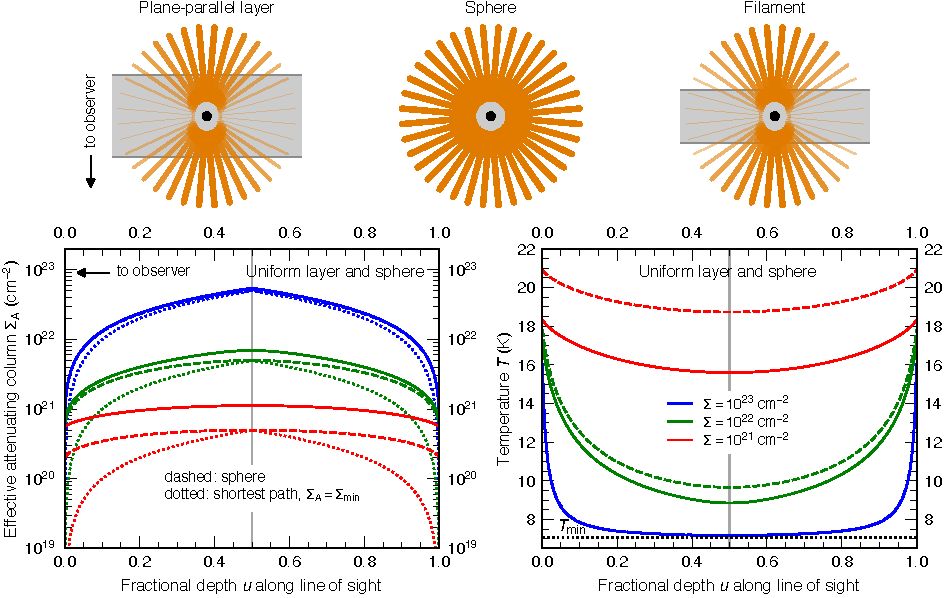
\includegraphics[width=0.85\linewidth]{fig_geometry.pdf}
\caption{Geometry of the dust attenuation in different structures. \emph{Upper}: The radiation that heats a dust grain (black
point) arrives from every direction after crossing very different columns. The rays are thicker where less material has been
crossed. Most energy arrives along the normal in the midplane of a layer, and no direction is favored at the center of a sphere. A
cylindrical filament resembles a layer along its axis and a sphere across the axis. \emph{Lower left}: The effective attenuating
column $\Sigma_{\rm A}$ of Eq.~(\ref{eq:seff}) against the fractional depth $u$ along the line of sight normal to a uniform layer
(solid curves) and along the diameter of a uniform sphere (dashed curves), for $\Sigma = 10^{21}$, $10^{22}$, and
$10^{23}$\,cm$^{-2}$. The dotted curves show the column $\Sigma_{\rm min} = \min(u, 1-u)\,\Sigma$ along the shortest path to the
surface. The thin vertical line marks the midplane of the layer and the center of the sphere. \emph{Lower right}: The dust
temperature that follows from $\Sigma_{\rm A}$ through Eq.~(\ref{eq:law}). The dotted line marks the floor temperature
$T_{\rm min}$.}
\label{fig:geometry}
\end{figure*}

\subsection{Diffuse cloud and simulated star-forming region}
\label{sec:modcloud}

Most of the observed area of a molecular cloud is covered by extended diffuse material, referred to here as the diffuse cloud, or
simply the cloud. It was modeled as a rectangular box of $6.8{\times}6.8$\,pc with a $2$\,pc depth along the line of sight. Its
projection was a surface density map with scale-free fluctuations and with an enhancement toward the center
(Fig.~\ref{fig:cube3d}). The map was derived from the same scale-free background used previously in
\citet{Menshchikov_etal2012,Menshchikov2021method,Menshchikov2021bench}. The volume density was constructed to fluctuate along
every line of sight with the same power spectrum as across the sky (Appendix~\ref{app:simcloud}). Its surface densities were
$3{\times}10^{20}$--$3{\times}10^{22}$\,cm$^{-2}$, with a median of $5{\times}10^{21}$\,cm$^{-2}$.

The simulated star-forming region combined this cloud with seven filaments and $96$ cores in an image of $1793{\times}1793$ pixels
of $3{\arcsec}$. Every structural component was computed with the radiative transfer code, so that its emission and its surface
density were consistent. The filaments and the cores were the models embedded in cylindrical and spherical envelopes
(Sects.~\ref{sec:modfil} and \ref{sec:modcores}), with the emission of the envelopes subtracted. The envelopes were matched to the
simulated cloud at the positions of the structures, so that the filaments and the cores were shielded approximately as at the
middle depth of the cloud (Appendices~\ref{app:embfil} and \ref{sec:grid}).

The emission of the simulated star-forming region was convolved to the beams of the wavebands at $160$--$500${\um} and its surface
density $\Dim_{13.5}$ was derived with \emph{hires}, as done for real observations. The true surface density was also convolved to
the same resolution.

% =====================================================================

\section{Radiation shielding and dust temperature}
\label{sec:law}

Dust in molecular clouds is heated mostly by the interstellar radiation field that arrives from outside the clouds, and locally
also by young stars formed within them. The temperature of a dust grain is set by the amount of radiation that reaches it. The
models and the correction of this paper consider the external heating only, for which this amount is reduced by the material
between the grain and the outside of the cloud. Internal heating is discussed in Appendix~\ref{sec:notdo}.

\subsection{Effective attenuating column}
\label{sec:why}

The external radiation arrives from all directions, and it crosses different amounts of material in each direction. Let $I_{\lambda
0}$ be the unattenuated radiation field at a wavelength $\lambda$. Denoting $\Sigma(\hat{n})$ the column of hydrogen molecules
(cm$^{-2}$) that the radiation crosses on its way in along the direction $\hat{n}$, the mean intensity $J_{\lambda}$ that reaches
the grain is
\begin{equation}
  J_{\lambda} = \frac{1}{4\pi} \int_{4\pi} I_{{\lambda}0}\,\exp\left(-\sigma_{\lambda}\,\Sigma(\hat{n})\right){\rm d}\Omega,
\label{eq:meanint}
\end{equation}
where $\sigma_{\lambda}$ is the extinction cross section per hydrogen molecule. The quantity $\Sigma(\hat{n})$ is the attenuating
column in the direction $\hat{n}$.

Figure~\ref{fig:geometry} illustrates this for the three shapes used to describe structures in clouds. Deep inside
a layer, the radiation arrives almost entirely along the normal. A direction inclined by an angle $i$ crosses $(\cos i)^{-1}$ times
more material, and grazing directions deliver nothing. At the center of a sphere, every direction crosses the same column, and no
direction is preferred. A straight filament resembles a sphere across its axis and a layer along it.

The mean intensity of Eq.~(\ref{eq:meanint}) is an integral over all directions, each with its own column $\Sigma(\hat{n})$. It is
convenient to describe the shielding of a dust grain by a single number instead, as the column that would give the same mean
intensity if it were the same in all directions. With a gray cross section $\sigma$ (see below), this effective attenuating column
$\Sigma_{\rm A}$ is defined by
\begin{equation}
  \Sigma_{\rm A} = - \frac{1}{\sigma}
    \ln \left\langle\,\exp\left({-\sigma\,\Sigma\!\left(\hat{n}\right)}\right)\,\right\rangle_{4\pi},
\label{eq:seff}
\end{equation}
where the angle brackets denote averaging over all directions. The exponential describes the fraction of the external radiation
that reaches the grain from the direction $\hat{n}$. For an isotropic external field, the average of this fraction over all
directions is the ratio $J_{\lambda}/I_{\lambda 0}$ of Eq.~(\ref{eq:meanint}), so that $\sigma\Sigma_{\rm A} = -\ln
\left(J_{\lambda}/I_{\lambda 0}\right)$ is the optical depth that would reduce the radiation reaching the grain by that factor.

This average in Eq.~(\ref{eq:seff}) is dominated by the least shielded directions, because the exponential suppresses the
contribution of heavily shielded ones. For an infinite layer, the arithmetic mean of $\Sigma(\hat{n})$ is infinite, whereas
$\Sigma_{\rm A}$ remains finite. At the other extreme is the column along the shortest path to the surface, $\Sigma_{\rm min} =
\min_{\hat{n}}\Sigma(\hat{n})$. No exponential in Eq.~(\ref{eq:seff}) exceeds $\exp(-\sigma\Sigma_{\rm min})$, so $\Sigma_{\rm A}
\ge \Sigma_{\rm min}$, with equality only if all the radiation arrived from the least shielded direction. Deep inside a structure
the two nearly agree, because only the directions close to the shortest path still deliver radiation. Near a surface they differ
most. At the surface of an optically thick layer $\Sigma_{\rm min} = 0$, whereas half of the directions are blocked, so that
$\sigma\Sigma_{\rm A} = \ln 2$ and $\Sigma_{\rm A} \approx 7{\times}10^{20}$\,cm$^{-2}$. Figure~\ref{fig:angular} shows how the
average of Eq.~(\ref{eq:seff}) is formed at the midplane of a layer, and how $\Sigma_{\rm A}$ grows with the total surface density
of the line of sight.

The above reasoning contains two simplifications. First, the radiation field outside the cloud was assumed to be isotropic, that
is, the same in all directions $\hat{n}$, as in all the models (Sect.~\ref{sec:models}). Second, the extinction across the
ultraviolet and optical wavelengths was assumed to be gray, with $A_{V} = \Sigma / (0.94{\times}10^{21}\,{\rm cm}^{-2})$
\citep{Bohlin+1978} and the optical depth $\tau = A_{V} / 1.086 = \sigma\,\Sigma$, where $\sigma = 9.8{\times}10^{-22}$\,cm$^{2}$.
In reality, the extinction decreases with wavelength, so the effective cross section decreases with depth, where the radiation is
redder. A constant gray cross section is adequate, because the relation between $T$ and $\Sigma_{\rm A}$ was fitted to the
radiative transfer models (Sect.~\ref{sec:relation}), computed with the full wavelength dependence of the opacity.

\begin{figure}
\centering
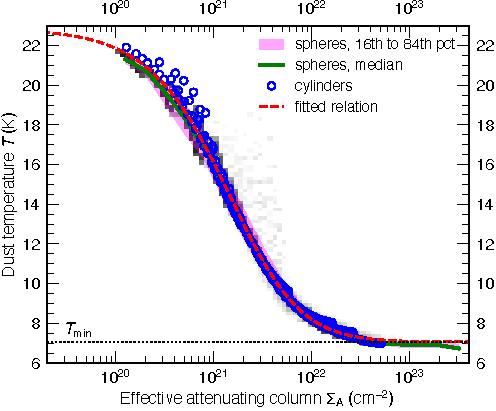
\includegraphics[width=0.93\columnwidth]{fig_shielding.pdf}
\caption{The dust temperature against the effective attenuating column $\Sigma_{\rm A}$ in the radiative transfer models. The gray
scale shows the distribution of the radial shells (over $10^5$) of the $2086$ spheres in this plane, each shell weighted by its
mass, with every sphere given the same total weight. The gray scale is logarithmic and spans four orders of magnitude. The green
solid line and the magenta band are, respectively, the weighted median and the 16th to 84th percentiles of the temperature in bins
of $0.2$\,dex in $\Sigma_{\rm A}$. The blue circles correspond to the $45$ radii of each of the seven cylinders. The red dashed
line is the relation of Eq.~(\ref{eq:law}), fitted to the spheres and the cylinders with equal total weights. The dotted line marks
the temperature $T_{\rm min}$ that fully shielded dust approaches.}
\label{fig:shielding}
\end{figure}

\subsection{Dependence of dust temperature $T$ on $\Sigma_{\rm A}$}
\label{sec:relation}

%%%%% -----------------------------------------------------------------------------------------------------------------------------
%%%%% NUMBERS (2026-10-20): 2.4 K is the mass-weighted mean excess over the relation of the outermost shells of the spheres in the
%%%%% densest embedding clouds (cSD_09), measured on attenuation_law.txt of the fit with the outermost shells kept (-keepouter);
%%%%% the shells were identified with the node column of the table and diagnose_shielding_branches.py.
%%%%% -----------------------------------------------------------------------------------------------------------------------------
The relation between $\Sigma_{\rm A}$ and $T$ follows from radiative transfer, once the dust properties and the external radiation
field are fixed. The density and the dust temperature of every model are tabulated in radial shells, the cells of its radial grid:
spherical shells for the cores and cylindrical shells for the filaments. The attenuating column of a shell was computed by
integrating the number density of hydrogen molecules along many rays, $240$ directions for the cores and $200{\times}180$
directions of equal solid angle for the filaments, and Eq.~(\ref{eq:seff}) was then evaluated by summing over the directions. A few
innermost shells of the densest cores, with poor Monte Carlo statistics, and the outermost shell of every sphere, whose single
temperature is an average over a steep gradient, were rejected (Appendix~\ref{sec:grid}).

%%%%% -----------------------------------------------------------------------------------------------------------------------------
%%%%% NUMBERS (2026-10-20): T_min, T_max, Sigma_star, gamma and the scatter from the header of attenuation_law.txt written by
%%%%% fit_attenuation_law.py (2086 spheres without their outermost shells, 7 isolated cylinders, equal weights). The departures
%%%%% of the spheres and cylinders and the leave-one-cylinder change of the factor from python/paper_numbers/law_checks.py with
%%%%% attenuation_law.txt and attenuation_law-leave_one_cylinder_out.txt (the seven fits run with fit_attenuation_law.py,
%%%%% one cylinder left out each).
%%%%% -----------------------------------------------------------------------------------------------------------------------------
More than $10^5$ shells of the $2086$ spheres and $45$ shells of each of the seven cylinders follow a single relation
(Fig.~\ref{fig:shielding}) that can be fitted with the function
\begin{equation}
  T(\Sigma_{\rm A}) = T_{\rm min} + \left(T_{\rm max} - T_{\rm min}\right) \left(1 + \Sigma_{\rm A}/{\Sigma_\star}\right)^{-\gamma},
\label{eq:law}
\end{equation}
where the fit parameters are $T_{\rm min\!} = 7.0495$\,K, $T_{\rm max\!} = 22.8668$\,K, $\Sigma_{\star\!} =
2.3897{\times}10^{21}$\,cm$^{-2}$, and $\gamma = 1.5969$. The fit minimized the mass-weighted sum of the squared logarithmic
differences between the fitted and the model temperatures, with every sphere and every cylinder normalized to the same total weight
and the two types of structure given equal weights. The mass-weighted scatter about the relation is $2.4$\%. The cores and the
filaments follow the same relation: on average, the cores are $0.6$\% colder than the relation and the filaments $0.1$--$1.1$\%
warmer. Leaving out any single filament changes the correction factor by at most $1.5$\%. Above $\Sigma_{\rm A\!}\approx
10^{23}$\,cm$^{-2}$, the models contain too little mass to constrain the relation.

\begin{figure*}
\centering
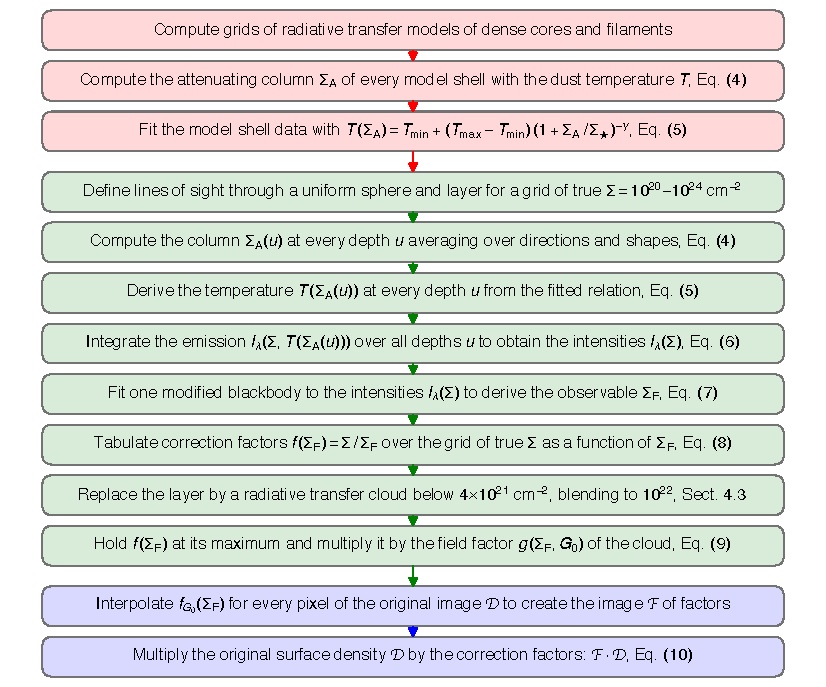
\includegraphics[width=0.75\textwidth]{fig_method.pdf}
\caption{Flowchart of the method. The first group is the calibration, which is done once and yields the temperature relation of
Eq.~(\ref{eq:law}). The second is the calculation of Sect.~\ref{sec:factor}, repeated for a grid of true surface densities
$\Sigma$, which yields the table of the correction factor against the surface density that an observed image actually holds. Its
last two steps calibrate the low surface densities on a radiative transfer model of a diffuse cloud (Sect.~\ref{sec:diffuse}) and
adapt the factor to the radiation field of the cloud (Sect.~\ref{sec:g0corr}). The third group is what is then done to an image, at
any resolution.}
\label{fig:method}
\end{figure*}

The two limits have simple meanings. $T_{\rm max}$ is the temperature of dust that the radiation reaches without attenuation.
$T_{\rm min}$ is the temperature that dust approaches when the ultraviolet and optical radiation no longer reach it. The dust is
then heated only by the infrared radiation that still penetrates, including the emission of the warmer dust around it, and by the
cosmic microwave background. Between the two limits, $\Sigma_\star$ is the characteristic attenuating column of the decline: at
$\Sigma_{\rm A\!} = \Sigma_\star$, the excess of the temperature over $T_{\rm min}$ is reduced by the factor $2^{\gamma\!}\approx
3$, and $\gamma$ sets how steeply the temperature falls at larger columns.

The size and the concentration of a core do not appear in Eq.~(\ref{eq:law}), because they affect $T$ only by changing the amount of
material between the dust and the radiation. For the same reason, the filaments did not need a surrounding cloud, because
$\Sigma_{\rm A}$ of every dust grain already includes all the material that shields it. Accordingly, the cores, embedded in
envelopes that differ by a factor of $256$ in $\Sigma$, follow the same relation. An isolated cylinder provides the shielding
geometry of a
filament without an artificial envelope, which shields the axis less than a cloud layer of the same $\Sigma$
(Appendix~\ref{app:embfil}). The scatter of $2.4$\% reflects the physics that a single gray $\Sigma_{\rm A}$ omits, mainly the
wavelength dependence of the
extinction, and it would not decrease with more models.

% =====================================================================

\section{The correction method}
\label{sec:corr}

\subsection{The correction factor for uniform structures}
\label{sec:factor}

The correction factor $f$ is the ratio of the true surface density $\Sigma$ of a line of sight to the surface density $\Sigma_{\rm
F}$ obtained by fitting a single-temperature modified blackbody to the intensities $I_{\lambda}$ emerging along it. It was computed
for a grid of $\Sigma$, $10^{20}$--$10^{24}$\,cm$^{-2}$ in logarithmic
steps. Apart from the calibration of diffuse material (Sect.~\ref{sec:diffuse}), the derivation has no free parameters.

Calculating $f$ requires a model of the distribution of the material along the line of sight. Two bodies of uniform density with
the same surface density $\Sigma$ were adopted: a sphere, seen through its center, and a plane-parallel layer, seen along its
normal. Each line of sight was divided into short segments. The position of a segment is given by $u$, which is the fraction of
$\Sigma$ that lies in front of it, from $u = 0$ at the near surface to $u = 1$ at the far surface. The factor was computed in five
steps (Fig.~\ref{fig:method}).

(1) The effective attenuating column $\Sigma_{\rm A}$ of every segment was computed from Eq.~(\ref{eq:seff}), separately for the
sphere and the layer. The two values were averaged for each segment, for the reason given in Sect.~\ref{sec:orient}, giving a
single profile $\Sigma_{\rm A}(u)$ for the line of sight.

(2) The dust temperature of every segment followed from $\Sigma_{\rm A}(u)$ and the relation of Eq.~(\ref{eq:law}). The
temperature is therefore highest at the two surfaces of the line of sight and lowest in its middle, where $\Sigma_{\rm A}$ is
largest.

(3) The intensity $I_{\lambda}$ emerging from the line of sight was obtained by integrating the emission of all its segments,
\begin{equation}
   I_\lambda(\Sigma) = \kappa_\lambda\,\eta\,\muH\,\mH\,\Sigma \int_0^1 B_\lambda \big(T(\Sigma_{\rm A}(u))\big)\,{\rm d}u,
\label{eq:emission}
\end{equation}
where $\kappa_\lambda$ is the dust opacity per unit mass of dust, $\eta = 0.01$ is the dust-to-gas mass ratio, $\muH = 2.8$ is the
mean molecular weight per hydrogen molecule, and $\mH$ is the mass of a hydrogen atom.

(4) A single modified blackbody was fitted to these intensities exactly as \emph{hires} fits the observed images: in the same
wavebands, $160$--$500${\um}, and with the same weights, inversely proportional to the squares of the calibration
uncertainties, $20$\% at $160${\um} and $10$\% at $250$--$500${\um} \citep{Konyves+2015}. The fit gave a temperature $T_{\rm F}$,
and the surface density $\Sigma_{\rm F}$ for this line of sight was derived from the intensity $I_{\rm ref}$ at the reference
wavelength $\lambda_{\rm ref\!}=500${\um}, at which $\Sigma_{\rm F}$ is least sensitive to the temperature (cf.
Eq.~(\ref{eq:sensitivity})):
\begin{equation}
   \Sigma_{\rm F}(\Sigma) = \frac{I_{\rm ref}(\Sigma)} {\kappa_{\rm ref}\,\eta\,\muH\,\mH\,B_{\rm ref}(\Teff)}.
\label{eq:fitted}
\end{equation}
Below, $T_{\rm F}$ and $\Sigma_{\rm F}$ are called the fitted temperature and the fitted surface density, the values that a
single-temperature fit returns.

(5) The correction factor is the ratio of the true and fitted surface densities. An observed image contains $\Sigma_{\rm F}$, not
$\Sigma$, so the factor was tabulated against $\Sigma_{\rm F}$:
\begin{equation}
   f(\Sigma_{\rm F}) = {\Sigma}/{\Sigma_{\rm F}}.
\label{eq:factor}
\end{equation}

\begin{figure}
\centering
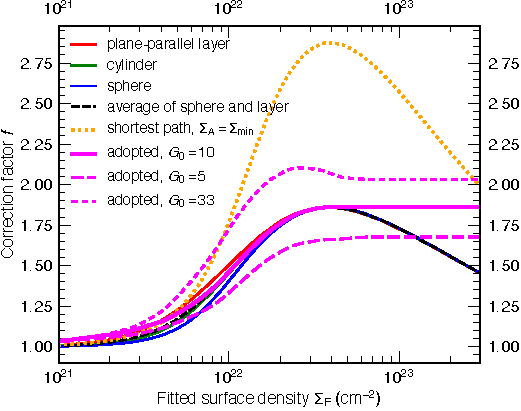
\includegraphics[width=0.96\columnwidth]{fig_relation.pdf}
\caption{The correction factor as a function of the surface density $\Sigma_{\rm F}$ of the uncorrected image for three uniform
structures -- plane-parallel layer, cylinder, and uniform sphere -- and for an average of the sphere and layer, with $G_0 = 10$.
The dotted curve shows the factor when the column $\Sigma_{\rm A}$ is replaced with $\Sigma_{\rm min}$ along the shortest path
instead of the angular average (Sect.~\ref{sec:why}); above $10^{22}$\,cm$^{-2}$ it overestimates the correction by up to $50$\%.
The thick magenta curve is the adopted relation for $G_0 = 10$. Below $3.98{\times}10^{21}$\,cm$^{-2}$ it replaces the analytic
layer by a radiative transfer model of a diffuse cloud (Sect.~\ref{sec:diffuse}), and above its maximum it is held constant
(Sect.~\ref{sec:factor}). The thin magenta curves are the adopted relation for $G_0 = 5$ and $33$, with the field factor of
Eq.~(\ref{eq:factorg0}).}
\label{fig:relation}
\end{figure}

Figure~\ref{fig:relation} shows the result. For the analytic structures, the factor is unity below $10^{21}$\,cm$^{-2}$, where
nothing is attenuated. It rises steeply through the range of surface densities of most of a molecular cloud. It reaches its
maximum, $1.86$, near $4{\times}10^{22}$\,cm$^{-2}$ and then declines, to $1.45$ at $3{\times}10^{23}$\,cm$^{-2}$. The factor is
largest when a line of sight contains both a warm surface layer, which dominates the emission, and a cold interior that holds most
of the mass. The surface layer has a nearly fixed surface density of a few $10^{21}$\,cm$^{-2}$, set by the depth to which the
heating radiation penetrates. Up to about $4{\times}10^{22}$\,cm$^{-2}$, the cold interior grows with $\Sigma$, and so does the
bias of the fit. At higher surface densities, most of the material of a uniform body has reached the temperature floor $T_{\rm
min}$. The cold interior then dominates the emission as well as the mass, $T_{\rm F}$ approaches $T_{\rm min}$, and the line of
sight becomes nearly isothermal again, so the factor declines toward unity.

Real dense structures are not uniform. A concentrated core has a cold center inside warmer outer layers, and its temperature still
varies along the line of sight. The radiative transfer models confirm this: the factor that they require stays between $2.0$ and
$2.4$ up to the highest surface densities of the models, ${\sim}10^{23}$\,cm$^{-2}$. The decline of the analytic relation is an
artifact of the uniform bodies. The factor was therefore held at its maximum above the surface density at which it is reached, so
that it never decreases with the surface density. The adopted relation differs from the analytic one in this respect and below
$10^{22}$\,cm$^{-2}$, for the reason given in Sect.~\ref{sec:diffuse}.

\subsection{Weak dependence on shapes and density distributions}
\label{sec:orient}

The correction factor assumes specific shapes of structures, however those in an observed region are unknown. Cores are embedded in
filaments, filaments are curved and blended with their neighbors, and everything lies in a fluctuating background. Fortunately, the
surface density correction depends little on the adopted shape.

Figure~\ref{fig:relation} shows the correction factor for a uniform sphere, cylinder, and plane-parallel layer of the same observed
surface density. The three agree to within $10$\% everywhere. Outside the range
$2.5{\times}10^{21}$--$1.3{\times}10^{22}$\,cm$^{-2}$, they agree to within $5$\%. This is because at low surface densities the
attenuation is weak, the
line of sight is nearly isothermal, and every shape gives $f \approx 1$. At high surface densities the deepest material is
optically thick in every direction, and the distribution of path lengths over directions no longer matters
(Fig.~\ref{fig:geometry}). Shapes of structures matter only in between, while the factor is still rising. This is why the
attenuating columns of the sphere and the layer were averaged in Sect.~\ref{sec:factor}, and half of the difference of their
factors, at most $5$\%, was regarded as the uncertainty due to the geometry.

A uniform cylinder seen perpendicular to its axis lies between the two limits, and its factor is within $1.5$\% of their average,
so the average also represents filaments. The factor was computed for central lines of sight, along the normal of a layer and the
diameter of a sphere. Off-center lines of sight through a sphere or a filament pass closer to its surface. They are warmer and more
nearly isothermal than a central line of sight with the same $\Sigma$, and they are slightly over-corrected. The validation on all
pixels of the models includes this effect (Sect.~\ref{sec:valgrid}). Inclined layers and filaments are over-corrected too
(Appendix~\ref{sec:incl}). Appendix~\ref{app:shape} shows that the sphere and the layer are the two extreme shapes.

One assumption remains: each structure was assumed to have a uniform density. For a plane-parallel layer, in which the density
varies only along the line of sight, this assumption does not matter. Radiation at an angle $i$ to the normal reaches a dust grain
at the depth $u$ through the column $u\,\Sigma/\cos i$ from the front face or $(1-u)\,\Sigma/\cos i$ from the back face, however the
material is distributed. Therefore, $\Sigma_{\rm A}$ and $T$ depend only on $u$ and $\Sigma$, and Eq.~(\ref{eq:emission}) holds for
any density profile. Two lines of sight with the same $\Sigma$ emit the same spectrum, whether their material is smooth or clumped.
Appendix~\ref{app:arrange} confirms this numerically, showing that density profiles
that differ by a factor of thirty reproduce the smooth case to within $0.02$\%.

This argument holds for a layer, in which radiation reaches the dust only through the material along the line of sight. In a
bounded structure, radiation also reaches the dust from the sides, and only through this effect do the concentration and
arrangement of the material matter. Their effect is modest. A sphere with a central-to-edge density ratio of $10$ needs a
correction $2$--$5$\% larger than a uniform sphere of the same central surface density. For a ratio of $10^3$, it needs $9$--$20$\%
more, and the difference grows with the surface density. A structure embedded at an unknown depth in a diffuse cloud is a
different case. In the extreme cases, the correction for such a line of sight is $13$\% too small, for a structure in a tenuous
cloud, or $21$\% too large, for a structure at a face of a dense cloud. These cases are not typical: near the middle of a cloud,
the error is only a few percent, and in the simulated star-forming region it is about $10$\% (Sect.~\ref{sec:sim}). Both effects
are measured in Appendix~\ref{app:arrange}, and they enter the uncertainties of Appendix~\ref{sec:limits}.

\subsection{Calibration on a diffuse cloud at low surface densities}
\label{sec:diffuse}

The relation of Eq.~(\ref{eq:law}) was determined for bounded structures (spheres and cylinders). Most of the area of molecular
clouds is covered by diffuse material, so the correction factor $f$ was also calibrated on the radiative transfer model of the
diffuse cloud (Sect.~\ref{sec:modcloud}). For each line of sight (pixel) of this model, one modified blackbody was fitted to the
intensities at $160$--$500${\um}, and the result was compared with the true surface density.

The analytic layer, which enters the average of Sect.~\ref{sec:orient}, does not reproduce the correction factors that the
radiative transfer model of the cloud requires. The layer needs almost no correction below $10^{21}$\,cm$^{-2}$, but the cloud
needs $5$\% even at $3.5{\times}10^{20}$\,cm$^{-2}$ and $15$--$25$\% at $2$--$4.5{\times}10^{21}$\,cm$^{-2}$. The reason is the
surface of the cloud, whose outer layers are heated by the unattenuated ultraviolet radiation from half the sky. They are up to
$3$\,K warmer than Eq.~(\ref{eq:law}) predicts, because that relation describes the attenuation with a single gray opacity. The
temperature therefore varies more along a line of sight through the cloud than through the analytic layer.

The analytic layer was therefore replaced by the radiative transfer model of the cloud at low $\Sigma_{\rm F}$. Below $\Sigma_{\rm
F} = 3.98{\times}10^{21}$\,cm$^{-2}$, $f$ was set to the average of $f$ of the analytic sphere and of $f$ measured on the cloud.
Between $3.98{\times}10^{21}$ and $10^{22}$\,cm$^{-2}$, it was blended smoothly into the analytic average of
sphere and layer, which was used above. Extending the calibration on the cloud to higher surface densities was tested and rejected:
it improved the cloud by only $2$\%, did not improve the flanks of the dense filaments in the simulated star-forming region, and
over-corrected dense cores. The factor remains a function of the surface density alone. The bounded spheres and the extended cloud
are the two limits for diffuse material, as the sphere and the layer are for a single structure. Their average divides the
uncertainty between them. As a result, the uniform envelopes of the cores are corrected about $2$\% too much and the model of the
diffuse cloud $11$\% too little in the median (Sects.~\ref{sec:valgrid} and \ref{sec:sim}).

\subsection{Adaptation to different radiation fields}
\label{sec:g0corr}

The relation of Eq.~(\ref{eq:law}) and the correction factor $f$ were calibrated for $G_0 = 10$. However, different clouds are
heated by radiation of very different strengths. The diffuse material of the molecular clouds listed in Appendix~\ref{app:fieldest}
requires fields $G_0 \lesssim 1$--${\sim}250$. A stronger field heats the dust at every attenuating column, and it changes
the temperature contrast along the line of sight, of which $T_{\rm max}/T_{\rm min}$ is the largest value.
The factor that a line of sight requires therefore depends on the
field (Appendix~\ref{sec:field}).

This dependence was measured on the model grid of embedded cores (Sect.~\ref{sec:modcores}) for nine radiation fields $G_0 =
0.98$--$483$. For each field, the pixels of all its models were binned in their true surface density, and the mean logarithm of
the factor that each bin required gives, with the mean $\log\Sigma_{\rm F}$ of the bin, the mean factor as a function of
$\Sigma_{\rm F}$ (Appendix~\ref{app:fieldR}). The ratio of this mean to the same mean at $G_0 = 10$ defines the field factor
$g(\Sigma_{\rm F}, G_0)$ (Fig.~\ref{fig:fieldfactor}). Above $7.1{\times}10^{22}$\,cm$^{-2}$, the grid contains too few pixels to
determine it, and $g$ was held at its value there. Between the radiation fields, $\log g$ is interpolated linearly in $\log G_0$.
The field factor is close to unity in diffuse material and departs from it most above ${\sim}10^{22}$\,cm$^{-2}$. It is largest for
$G_0 \approx 50$, and in the strongest fields it falls below unity at high surface densities (Appendix~\ref{app:field}).

\begin{figure}
\centering
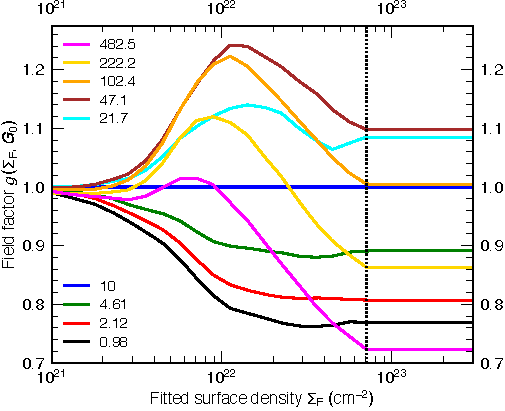
\includegraphics[width=0.96\columnwidth]{fig_fieldfactor.pdf}
\caption{The radiation field factor $g(\Sigma_{\rm F}, G_0)$ from Eq.~(\ref{eq:factorg0}) is plotted against the fitted surface
density $\Sigma_{\rm F}$, for the nine field strengths $G_0$ of the model grid, from the weakest to the strongest. For the field
$G_0 = 10$ of the calibration, $g = 1$. Above $7.1{\times}10^{22}$\,cm$^{-2}$ (dotted line), $g$ is held constant.}
\label{fig:fieldfactor}
\end{figure}

The surface density correction factor for a cloud in the radiation field with $G_0$ is
\begin{equation}
  f_{G_0}(\Sigma_{\rm F}) = g(\Sigma_{\rm F}, G_0) \,\max_{\Sigma^{\prime} \le \Sigma_{\rm F}} f(\Sigma^{\prime}),
\label{eq:factorg0}
\end{equation}
where the maximum holds the factor for uniform bodies at its maximum (Sect.~\ref{sec:factor}). The field factor is not held at its
maximum (Fig.~\ref{fig:fieldfactor}), because its decline in strong fields is measured on the radiative transfer models. The field
strength $G_0$ is a single number for a cloud. It is the value that the models require to reproduce the observed temperatures, an
effective field for the model dust, which can differ from the physical field. It is estimated from the temperatures of the diffuse
material of the whole map, with the procedure of Appendix~\ref{app:fieldest}. It is not read from the temperature of each pixel,
which is ambiguous (Appendix~\ref{app:tcorr}). The correction therefore still depends on the surface density alone, and the field
is an input of the method, like the wavebands.

\subsection{Correcting surface density images}
\label{sec:apply}

An observed surface density image is corrected by multiplying it by the image of the correction factors computed from the image
itself,
\begin{equation}
  \Dimc = \mathcal{F}\,\Dim, \quad \mathcal{F} \equiv f_{G_0\!}\left(\Dim\right),
\label{eq:correction}
\end{equation}
where $f_{G_0\!}$ of Eq.~(\ref{eq:factorg0}) is evaluated pixel by pixel. The corrected image $\Dimc$ implies a temperature image
$\mathcal{T}_{\rm C}$ with lower dust temperatures, at which $\Dimc$ gives the same intensities at $500${\um} as $\Dim$ with the
fitted temperatures $\mathcal{T}$. By design, the correction factor is a function of only two quantities, the surface density of a
pixel and the radiation field strength $G_0$. The factor $f$ is analytic and does not depend on the angular resolution, whereas
the field factor $g$ and the temperatures used to estimate $G_0$ were measured on the images $\Dim_{13.5}$. When no estimate of
$G_0$ is supplied, the default $G_0 =
10$ is used. This paper uses the images $\Dim_{13.5}$, the finest that are usually available in practice. The resolutions of $8.4$
and $9.4{\arcsec}$ come from the images at $70$ and $100${\um}, which are usually too noisy in cold molecular clouds, although in
bright regions such as Cygnus~X even $\Dim_{8.4}$ is of good quality.

The correction method applies to surface density images at any angular resolution. The \emph{hires} images of the models of the
subdivision grid (Sect.~\ref{sec:modcores}) at $O = 8.4$, $9.4$, $13.5$, $18.2$, $24.9$, and $36.3{\arcsec}$ ($\Dim_{8.4}$ to
$\Dim_{36.3}$) were each corrected with their own factors $\mathcal{F}_{8.4}$ to $\mathcal{F}_{36.3}$. In all of them, the
correction restores the median total surface density to $0.99$--$1.00$ of the truth and the median core mass to $0.94$--$1.02$. The
factors evaluated on a coarser image give lower masses: applied to $\Dim_{13.5}$, the factors $\mathcal{F}_{36.3}$ give core masses
$5$\% lower than $\mathcal{F}_{13.5}$, and a larger underestimation at the core centers (Table~\ref{tab:valgrid}). On the cloud of
the simulated star-forming region, the two agree within $0.5$\%. The factor is therefore evaluated on the image that is corrected.
These tests
were made for $G_0 = 10$, so the field factor $g$ was not tested at other resolutions.

What \emph{hires} adds, and no correction can replace, is the information on scales smaller than the beam of the longest waveband.
Only the final images produced by \emph{hires} can be corrected, not the intermediate ones, because the latter are fitted to fewer
wavebands. The correction method is a \emph{Fortran} utility \emph{hicorrect} belonging to the source and filament extraction
method \emph{getsf} and is available on its webpage\footnote{\url{http://irfu.cea.fr/Pisp/alexander.menshchikov/}}.

\subsection{Requirements of the correction method}
\label{sec:needs}

The order of operations matters when an image is separated into its structural components, such as sources, filaments, and their
backgrounds \citep[e.g., with \emph{getsf},][]{Menshchikov2021method}. A dust grain is shielded by the whole column along its line
of sight, so the correction factor must be evaluated on the total surface density, not on a component of it. The image must
therefore be corrected first, and the components separated afterwards. If a background is subtracted first, the factor is evaluated
at a surface density that the material does not have, and the structure is corrected much too little. For the same reason, the
correction must never be applied to an image that is already corrected, or to a true surface density.

One condition applies when the correction is used outside \emph{hires}. The correction factor $f$ of Eq.~(\ref{eq:factor}) is built
for the wavebands and the weights of the fit (Sect.~\ref{sec:factor}), because $\Sigma_{\rm F}$ depends on both. For uniform
bodies, a map fitted with equal weights is under-corrected by $6$--$15$\% above $10^{22}$\,cm$^{-2}$, one fitted without $160${\um}
is over-corrected by $12$--$24$\%, and one whose fit includes $70$ or $100${\um} is under-corrected by up to $40$\%. The relation
cannot be replaced by anything derived from the photometry itself, because the mixing of temperatures along a line of sight changes
the spectral shape by only a few percent (Appendix~\ref{app:colors}).

For images derived with other wavebands or weights, the code computes $f$ of the uniform sphere and layer (Sect.~\ref{sec:factor})
for the wavebands and weights given, and at low $\Sigma_{\rm F}$ it combines $f$ with a calibration on the cloud model
(Sect.~\ref{sec:diffuse}) computed for the same set:
$160$--$500${\um} with the standard or equal weights, $250$--$500${\um}, $100$--$500${\um} and $70$--$500${\um}. The field factor
was measured with the standard set only. For $160$--$500$ and $250$--$500${\um} it is accurate to within $5$\% in fields $G_0
\lesssim 50$ and to within $16$\% in the strongest fields. For sets that include $70$ or $100${\um}, the error reaches $17$\%. The
effects of noise and of calibration errors are discussed in Appendix~\ref{sec:calerr}.

% =====================================================================

\section{Validation of the method}
\label{sec:valid}

The method can be tested only on images whose true surface density is known. The correction was tested in three settings, all
computed with radiative transfer. They are a grid of cores embedded in uniform envelopes, a set of isolated filaments, and a
simulated
star-forming region, in which a cloud, filaments, and cores overlap along the lines of sight. All of them were computed for $G_0 =
10$, hence $g = 1$ in Eq.~(\ref{eq:factorg0}). The factor $f$ was held at its
maximum (Sect.~\ref{sec:factor}) in all these tests. The correction for other fields was tested separately, on the models from
which $g$ was derived (Appendix~\ref{app:fieldR}). The calibration on the diffuse cloud and the simulated star-forming region
exist only for $G_0 = 10$.

\subsection{Tests on the models of cores}
\label{sec:valgrid}

The correction was validated on the subdivision grid (Sect.~\ref{sec:modcores}) of $1815$ radiative transfer models of embedded
spherical cores, which were not used to fit the relation of Eq.~(\ref{eq:law}). The image $\Dim_{13.5}$ of each embedded core was
corrected with the factors $\mathcal{F}_{13.5}$ evaluated on that image and, for comparison, with the factors $\mathcal{F}_{36.3}$
evaluated on $\Dim_{36.3}$. The corrected images were compared with the true surface density at the same resolution.

Table~\ref{tab:valgrid} presents four quantities. The total surface density was integrated over the true model footprint, defined
as the area within the contour at $1$\% of the peak of the core in its true image at $O = 13.5{\arcsec}$. The core mass $M$ was
integrated after subtraction of the background, defined as the median surface density in a ring $15{\arcsec}$ wide just outside the
footprint. The mass could be measured for $1750$ of the models (Appendix~\ref{sec:grid}). Both are given as accuracy ratios, the
corrected value divided by the true one. The relative error of the corrected surface density is given at $3$ and $21{\arcsec}$
from the center of the core, and its radial profile is shown in Fig.~\ref{fig:valgrid}.

\begin{table}
%%%%% -----------------------------------------------------------------------------------------------------------------------------
%%%%% NUMBERS (2026-11-09, rerun with f held at its maximum, unchanged after rounding): Table tab:valgrid and the numbers of Sect. 5.1
%%%%% are from validate3_finRTlaw.txt, written by
%%%%% validate_calib3.py on the subdivision grid: rows 'hicorrect2, fine' (factor at 13.5 arcsec) and 'hicorrect2, coarse' (36.3);
%%%%% Center and 21 arcsec from the radial table at 3 and 21 arcsec; the footprint errors from the table of the misjudged footprint.
%%%%% -----------------------------------------------------------------------------------------------------------------------------
\caption{Validation of the correction method on the radiative transfer models of embedded spherical cores.}
\label{tab:valgrid}
\centering
\begin{tabular}{@{}l@{\hspace{6pt}}c@{\hspace{6pt}}c@{\hspace{6pt}}c@{\hspace{6pt}}c@{}}
\hline\hline
\noalign{\smallskip}
\,Image\tablefootmark{a} & Total\tablefootmark{b} & Core mass $M$\tablefootmark{c} &\!\! Center\tablefootmark{d} 
&\!\!\! $21{\arcsec}$\tablefootmark{e}\\
\noalign{\smallskip}
\hline
\noalign{\smallskip}
\,$\Dim_{13.5}$                     & 0.78 (0.56--0.93) & 0.63 (0.46--0.86) &\!\!\! $-0.44$ &\!\!\! $-0.21$\,\\
\,$\mathcal{F}_{13.5\,}\Dim_{13.5}$ & 0.99 (0.92--1.03) & 0.98 (0.75--1.11) &\!\!\! $-0.13$ &\!\!\! $0.02$\,\\
\,$\mathcal{F}_{36.3\,}\Dim_{13.5}$ & 0.98 (0.90--1.02) & 0.93 (0.70--1.08) &\!\!\! $-0.16$ &\!\!\! $0.01$\,\\
\noalign{\smallskip}
\hline
\end{tabular}
\tablefoot{These $1815$ models were not used to fit the relation of Eq.~(\ref{eq:law}).
\tablefoottext{a}{The images before the correction and after it, with $\mathcal{F}_{13.5}$ or $\mathcal{F}_{36.3}$.}
\tablefoottext{b}{The accuracy ratio of the total surface density over the true model footprint: the median over the models, with
the 16th and 84th percentiles in parentheses.}
\tablefoottext{c}{The accuracy ratio of the core mass, for the $1750$ models in which it can be measured: the median and
percentiles as in (b).}
\tablefoottext{d}{The median relative error of the surface density at $3{\arcsec}$ from the center of the core.}
\tablefoottext{e}{The same at $21{\arcsec}$ from the center.}
}
\end{table}

\begin{figure}
\centering
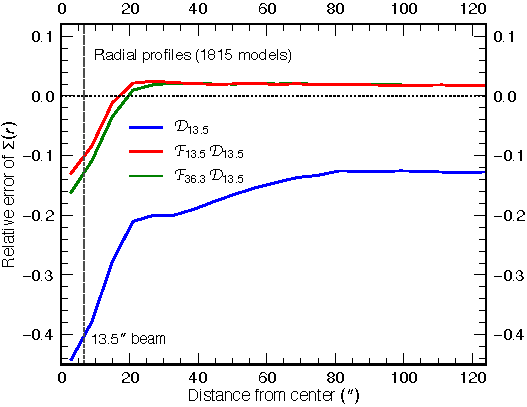
\includegraphics[width=0.96\columnwidth]{fig_grid_validation.pdf}
\caption{Testing the correction method on the radiative transfer models of embedded cores. The relative error of the corrected
surface density (Sect.~\ref{sec:valgrid}) is shown against the distance from the center of the core, as the median over the
$1815$ models. The dashed line marks $O/2$ for $O = 13.5{\arcsec}$.}
\label{fig:valgrid}
\end{figure}

The uncorrected $\Dim_{13.5}$ contains $78$\% of the true $\Sigma$ and $63$\% of the true $M$. The largest
underestimation, $44$\%, is at the core center. The correction restores the median total to $99$\% and the median $M$ to $98$\%.
Beyond $15{\arcsec}$ from the center, the corrected $\Sigma$ is overestimated by about $2$\% (Fig.~\ref{fig:valgrid}). There,
$\Sigma$ is
dominated by the uniform envelope of the core, which the calibration of Sect.~\ref{sec:diffuse}
corrects slightly too much. An underestimation of $13$\% remains at $3{\arcsec}$ from the centers of the cores. No correction that
depends on the surface density alone can remove it. The center of a core is colder than the center of a uniform structure with the
same $\Sigma$, and $\Sigma$ does not reveal this.

The errors of individual models are larger than the median errors. The corrected mass is underestimated by more than $25$\% for
one-sixth of the cores and overestimated by more than $11$\% for one-sixth (Table~\ref{tab:valgrid}). The errors depend on the
contrast of a core, the
ratio of its peak to the background. Cores with contrasts above $10$ dominate their lines of sight, and their cold interiors leave
the surface density at their centers underestimated by $45$\% and their masses by $16$\%. Cores with contrasts below $1.5$ are
nearly uniform, and their median mass is overestimated by $4$\%. No correction that depends on the surface density alone can remove
this
spread,
because cores with the same surface density differ in how their temperature varies along the line of sight. A footprint wrong by a
quarter of its radius changes the median mass by $-15$ to $+8$\%, much more than the correction leaves
(Appendix~\ref{app:footprint}).

\subsection{Tests on the models of filaments}
\label{sec:cyl}

The correction method was also validated on the seven radiative transfer models of isolated cylindrical filaments of
Sect.~\ref{sec:modfil}. Their surface density images $\Dim_{13.5}$, derived with \emph{hires} from the simulated emission, were
corrected with the factors $\mathcal{F}_{13.5}$ evaluated on them and compared with the true surface density at the same
resolution. They are isolated, so their profiles are not confused by any background. Table~\ref{tab:cyl} and
Fig.~\ref{fig:cylinders} give the results, measured on the median profile over the middle part of each cylinder.

\begin{table*}
%%%%% -----------------------------------------------------------------------------------------------------------------------------
%%%%% NUMBERS (2026-10-20): Table tab:cyl and the numbers of Sect. 5.2 from python/paper_numbers/cylinder_table.py on the seven
%%%%% *_isolated directories (mc.surfdens.fits and hi.surface.density.r13p5.fits; the factor is applied to the median profile,
%%%%% as in fig_cylinders).
%%%%% -----------------------------------------------------------------------------------------------------------------------------
\caption{Validation of the correction method on the radiative transfer models of isolated cylindrical filaments.}
\label{tab:cyl}
\centering
\begin{tabular}{@{}l@{\hspace{5pt}}cc@{\hspace{20pt}}cc@{\hspace{20pt}}ccc@{\hspace{20pt}}ccc@{}}
\hline\hline
\noalign{\smallskip}
\,\,$\Sigma_0$ (cm$^{-2}$)\tablefootmark{a} & \multicolumn{2}{c}{\!\!\!\!\!\!\!\!\!Crest\tablefootmark{b}} 
 & \multicolumn{2}{c}{\!\!\!\!\!\!\!\!$\Lambda$\tablefootmark{c}}
 & \multicolumn{3}{c}{\!\!\!\!\!\!\!\!$H_{13.5}$ (${\arcsec}$)\tablefootmark{d}}
 & \multicolumn{3}{c}{$\alpha_{13.5}$\tablefootmark{e}}\,\,\\
\noalign{\smallskip}
\cline{2-3}\cline{4-5}\cline{6-8}\cline{9-11}
\noalign{\smallskip}
\,\, & orig. & corr. & orig. & corr. & true & orig. & corr. & true & orig. & corr.\,\,\\
\noalign{\smallskip}
\hline
\noalign{\smallskip}
\,\,$3{\times}10^{21}$                  & 0.86 & 0.94 & 0.96 & 1.01 & 48 & 58          & 55 & 0.89 & 0.88 & 0.90\,\,\\
\,\,$1{\times}10^{22}$                  & 0.66 & 0.83 & 0.87 & 0.97 & 48 & 71          & 61 & 0.89 & 0.81 & 0.87\,\,\\
\,\,$3{\times}10^{22}$                  & 0.50 & 0.80 & 0.75 & 0.94 & 48 & 79          & 60 & 0.89 & 0.70 & 0.85\,\,\\
\,\,$5{\times}10^{22}$                  & 0.46 & 0.81 & 0.68 & 0.94 & 48 & 75          & 60 & 0.89 & 0.67 & 0.87\,\,\\
\,\,$1{\times}10^{23}$                  & 0.42 & 0.78 & 0.60 & 0.93 & 48 & 68          & 63 & 0.89 & 0.70 & 0.89\,\,\\
\,\,$3{\times}10^{22}$, $\beta=2$           & 0.50 & 0.80 & 0.73 & 0.93 & 47 & 72          & 57 & 1.07 & 0.86 & 1.02\,\,\\
\,\,$3{\times}10^{22}$, $H=80{\arcsec}$ & 0.53 & 0.88 & 0.71 & 0.95 & 85 &\!\!\!\! 122 & 92 & 0.80 & 0.59 & 0.76\,\,\\
\noalign{\smallskip}
\hline
\end{tabular}
\tablefoot{The seven filaments have $\beta = 1.75$ and intrinsic $H = 40{\arcsec}$, except where noted (cf. Table~\ref{tab:cylpar}),
and were convolved to $O = 13.5{\arcsec}$.
\tablefoottext{a}{The true surface density on the axis.}
\tablefoottext{b}{The accuracy ratio of the surface density on the axis, before and after the correction.}
\tablefoottext{c}{The accuracy ratio of the linear density within $\pm300{\arcsec}$, before and after the correction.}
\tablefoottext{d}{The half-maximum width of the true, the uncorrected, and the corrected profile.}
\tablefoottext{e}{The slope of $\log\Sigma$ against $\log r$ between $20$ and $120{\arcsec}$ from the crest, for the same three
profiles.}
}
\end{table*}

 \begin{figure*}
\centering
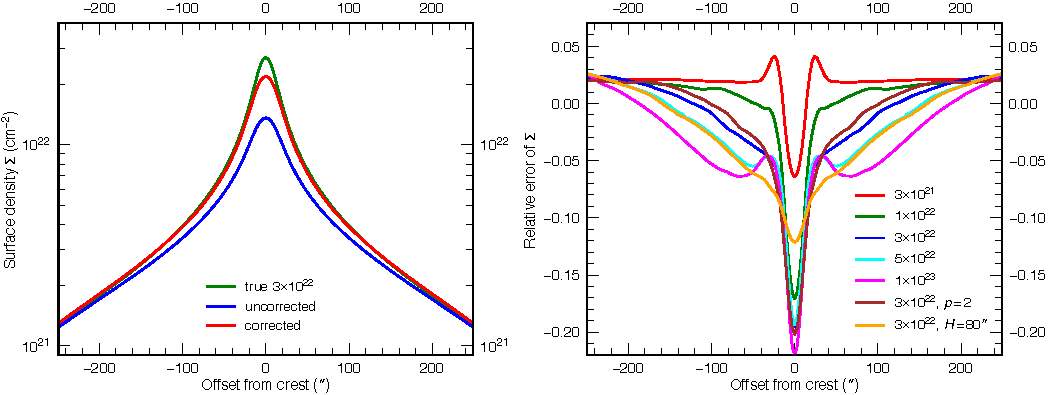
\includegraphics[width=\textwidth]{fig_cylinders.pdf}
\caption{The isolated radiative transfer cylinders reconstructed by \emph{hires} at $O = 13.5{\arcsec}$ and then corrected.
\emph{Left}: The profile across the cylinder with $3{\times}10^{22}$\,cm$^{-2}$ on its axis, true (convolved to the beam),
uncorrected and corrected. \emph{Right}: Relative error of the corrected surface density across all seven cylinders, labeled by
their surface density $\Sigma_{0}$ on the axis. Each profile is the median over the middle part of the cylinder.}
\label{fig:cylinders}
\end{figure*}

Without the correction, the crests of the filaments are underestimated by $14$\% for the least dense filament and by $58$\% for the
densest (Table~\ref{tab:cyl}), and the profiles are too wide and too shallow, because the crest is suppressed much more than the
wings (Fig.~\ref{fig:cylinders}). After the correction, the linear densities $\Lambda$ are within $7$\% of the truth and the slopes
$\alpha_{13.5}$ of the profiles within $0.05$. The crests remain underestimated by $6$--$22$\%, and the widths of the six filaments
with
$H_{13.5} = 48{\arcsec}$ (intrinsic $H = 40{\arcsec}$) are $15$--$31$\% too large, because the axis of a filament, like the
center of a core, is colder than the middle of a uniform structure with the same surface density. Beyond about $20{\arcsec}$ from
the crest, the corrected profiles are within $8$\% of the truth (Fig.~\ref{fig:cylinders}).

\subsection{Tests on the simulated star-forming region}
\label{sec:sim}

The cores and filaments model a single structure, in contrast to the observed molecular clouds. The simulated star-forming region
of Sect.~\ref{sec:modcloud} contains a cloud, seven filaments and $96$ cores, which overlap along the lines of sight. Its image
$\Dim_{13.5}$ was corrected with the factors $\mathcal{F}_{13.5}$ and compared with the true surface density at the same
resolution, as was the image of the same region with the cloud alone.

\begin{figure*}
\centering
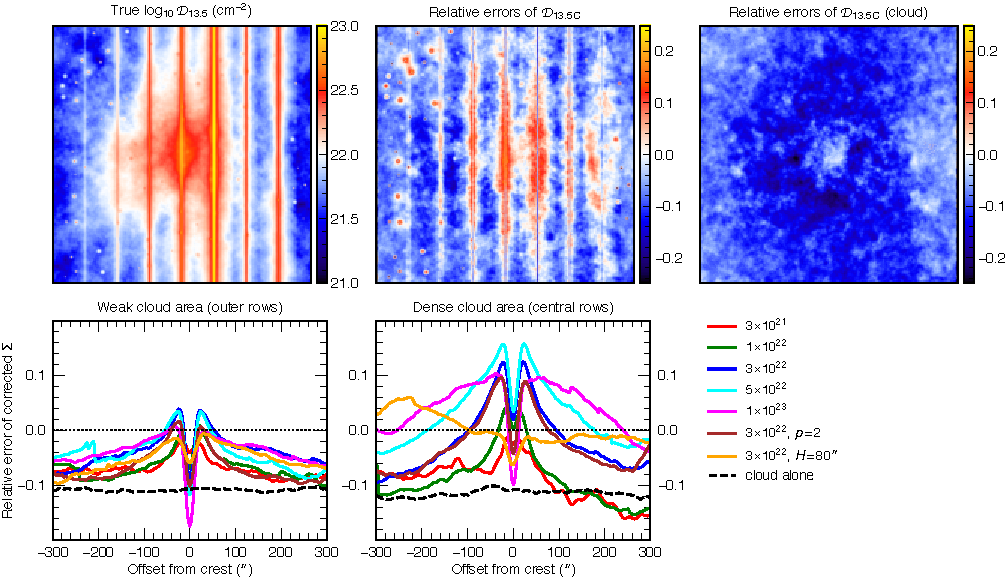
\includegraphics[width=\textwidth]{fig_simsky6.pdf}
\caption{The simulated star-forming region, built from radiative transfer models of a cloud, seven filaments and $96$ cores.
\emph{Upper left}: the true surface density at $O = 13.5{\arcsec}$. \emph{Upper middle}: the relative error of the corrected
surface density, (corrected $-$ true) / true. \emph{Upper right}: the same for a region that contains the cloud alone. \emph{Lower
panels}: the relative error across each filament, as the median over the outer rows of the region, where the cloud is tenuous, and
over its central rows, where the cloud is dense. The filaments are labeled by their surface density $\Sigma_{0}$ on the axis. The
cores are masked in the profiles. The dashed curve is the cloud alone at the same positions.}
\label{fig:simsky6}
\end{figure*}

%%%%% -----------------------------------------------------------------------------------------------------------------------------
%%%%% NUMBERS (2026-10-20): Sect. 5.3 from python/paper_numbers/simsky_numbers.py on simsky6_RT_enh_cirrdepth=2_nocrater (the sky),
%%%%% simsky6_RT_enh_cirronly (the cloud alone) and the core catalog simsky6.w40.cores.cores.txt. The crests, flanks and wings are
%%%%% read from the profiles at 0, 15-45 and 240 arcsec; the median accuracy ratio with the cores masked is 0.949 and 0.731 (corrected,
%%%%% uncorrected); the totals 0.98 and 0.67 are the ratios of the sums of corrected or uncorrected to true Sigma over the whole image
%%%%% without masking (recomputed on 2026-11-09 with hicorrect2.py; with the cores masked, 0.968 and 0.663).
%%%%% -----------------------------------------------------------------------------------------------------------------------------
Figure~\ref{fig:simsky6} shows the relative error of the corrected surface density over the region, for the cloud alone, and across
the filaments. For the cloud alone, the correction raises the median accuracy ratio of $\Sigma$ from $0.76$ to $0.89$. The corrected
$\Sigma$ is underestimated by $6$\% at $\Sigma = 10^{21}$\,cm$^{-2}$ and by $14$\% at $\Sigma = 10^{22}$\,cm$^{-2}$. The remaining
underestimation of
$\Sigma$ in the cloud is the price of the average of Sect.~\ref{sec:diffuse}, which gives half the weight to the sphere.

In the outer parts of the simulated region, the cloud has $\Sigma \approx 2$--$5{\times}10^{21}$\,cm$^{-2}$. There the crests of
the filaments are corrected to within $4$--$17$\%, and their flanks to within $5$\%. Their outer wings are corrected too little,
by $6$--$9$\%, as much as the cloud around them. In the center, the cloud reaches $\Sigma \approx
2$--$3{\times}10^{22}$\,cm$^{-2}$. There the flanks of the dense filaments are corrected too much, by $10$--$16$\%, while the
cloud alone at the same positions is corrected too little.

Both effects come from the superposition of two structures, which a correction based on the surface density alone treats as one.
They have the signs predicted in Appendix~\ref{app:arrange}: a structure in a tenuous cloud is under-corrected, and a structure in
a dense cloud is over-corrected. The central cloud of the simulated star-forming region is two to three times denser than the
background of the filaments in Aquila, which \emph{getsf} determines to be $6{\times}10^{21}$ to $10^{22}$\,cm$^{-2}$ at most. In a
region like Aquila, the over-correction of the filament flanks should therefore be at most about $10$\%. The total surface density
of the whole simulated star-forming region is corrected from $0.67$ to $0.98$ of the truth.

\subsection{Remaining errors}
\label{sec:base}

%%%%% -----------------------------------------------------------------------------------------------------------------------------
%%%%% NUMBERS (2026-10-20): from validate3_finRTlaw.txt.nodes.txt (validate_calib3.py, per node), the 926 nodes with a half radius
%%%%% r_h below 13.5 arcsec, row 'hicorrect2, fine': median and 16th percentile of the central residual, median and 84th percentile
%%%%% of the largest residual of the radial profile within 3 r_h.
%%%%% -----------------------------------------------------------------------------------------------------------------------------
Two kinds of structure are not corrected well by any correction that depends on the surface density alone. The first kind
is the centers of concentrated structures. The crests of filaments remain underestimated by $6$--$22$\%, and the centers of cores by
$13$\% in the median. Cores with
$H_{13.5} < 2\,O$ \citep[cf.][]{Menshchikov+Zhang2026}, representing half of the models of the grid, remain underestimated by $27$\%
at their centers in the median and by more than $56$\% for one-sixth of them. They are surrounded by a ring that is over-corrected
by
$5$\% in the median and, for one-sixth of them, by more than $16$\%, because the beam spreads their cold centers over an area of
lower surface density. The second kind is
superposed structures of very different temperatures, which are corrected too little or too much, by $10$--$20$\%
(Sect.~\ref{sec:sim}). Corrections that also read the fitted temperature do not help (Appendix~\ref{app:tcorr}).

% =====================================================================

\section{Application to the Aquila cloud}
\label{sec:aquila}

The correction method was applied to a $31\arcmin{\times}31\arcmin$ sub-region of the Aquila star-forming region (centered at RA
$277{\fdg}4765227$, Dec $-1{\fdg}9962943$) observed with \emph{Herschel} \citep{Andre+2010, Konyves+2015}. The high-resolution
surface density image $\Dim_{13.5}$ with $625{\times}625$ pixels of $3{\arcsec}$ was derived with \emph{hires} using the observed
images at wavelengths of $160$, $250$, $350$, and $500${\um}. The correction factor was evaluated on $\Dim_{13.5}$ and applied to
every pixel, including those toward protostars (Appendix~\ref{sec:notdo}).

The interstellar radiation field for the cloud was estimated by \emph{hicorrect} with the procedure of Appendix~\ref{app:fieldest},
from the diffuse material of the entire Aquila region, which contains $2.9{\times}10^{7}$ pixels. The observations require a field
strength $G_0 \approx 33$, with $G_0 = 25$ and $41$ from the 16th and 84th percentiles of the fitted temperature. Therefore, the
correction method used $G_0 = 33$ in Eq.~(\ref{eq:factorg0}), about three times the field adopted in the calibration of the method.

%%%%% -----------------------------------------------------------------------------------------------------------------------------
%%%%% NUMBERS (2026-10-20): Sect. 6 from python/paper_numbers/aquila_numbers.py on the images of hires/Aquila_cutout_g33
%%%%% (hicorrect2 with -g0=33); the values for G_0 = 10 are recomputed by the same script from hicorrect2.py.
%%%%% -----------------------------------------------------------------------------------------------------------------------------
The median correction factor over the sub-region is $1.70$. It lies between $1.21$ and $2.10$ for $98$\% of the pixels and reaches
its maximum of $2.10$ at $\Sigma\approx 3{\times}10^{22}$\,cm$^{-2}$, so the correction is significant everywhere in the image. The
total surface density of the image increases by a factor of $1.86$. With the calibration value $G_0 = 10$, the median factor would
be $1.45$ and the total would increase by a factor of $1.61$.

The distribution of surface densities in $\Dim_{13.5}$ changes more than the median factor suggests, because the correction factor
rises with $\Sigma$. The median surface density of the image increases from $9.7{\times}10^{21}$ to
$1.7{\times}10^{22}$\,cm$^{-2}$, and its 99th percentile from $5.6{\times}10^{22}$ to $1.1{\times}10^{23}$\,cm$^{-2}$. The numbers
of pixels with values above $10^{22}$, $3{\times}10^{22}$, and $10^{23}$\,cm$^{-2}$ increase by factors of $1.8$, $5.2$, and $8.1$.
This matters for any criterion based on a surface density threshold, such as that for star formation.

\begin{figure*}
\centering
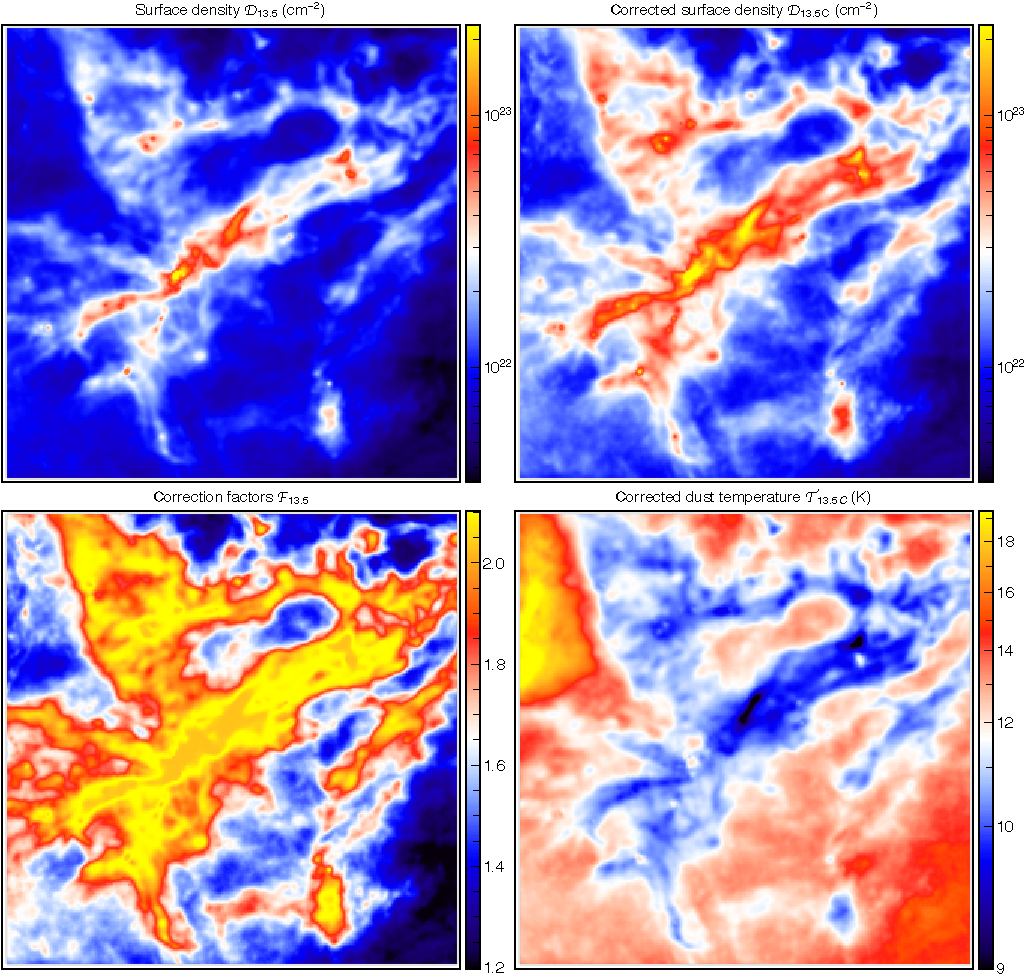
\includegraphics[width=0.98\textwidth]{fig_aquila.pdf}
\caption{The Aquila sub-region at $O = 13.5{\arcsec}$, corrected for the radiation field $G_0 = 33$. Shown are the images of the
surface density before and after the correction (on a common scale), of the correction factors, and of the corrected dust
temperature (Sect.~\ref{sec:aquila}). }
\label{fig:aquila}
\end{figure*}

Figure~\ref{fig:aquila} shows the images before and after the correction, together with $\mathcal{F}$ and $\mathcal{T}_{13.5\,\rm
C}$. The median for $\mathcal{T}_{13.5\,\rm C}$ is $12.2$\,K, against $15.0$\,K for the original $\mathcal{T}_{13.5}$, and its 1st
and 99th percentiles are $9.6$ and $18.6$\,K. The correction is not a uniform rescaling. The factor is smallest in the diffuse
material between the structures and largest along the crests of the filaments and at the cores. The correction therefore raises the
contrast of the image as well as its overall level. Above $\Sigma = 3{\times}10^{22}$\,cm$^{-2}$, the factor decreases slightly
from $2.10$ to $2.03$, so the densest crests and cores receive nearly the largest correction. The radiation field is not uniform
across the cloud. The warm corner in the upper left of $\mathcal{T}_{13.5\,\rm C}$ is heated more strongly than the rest of the
sub-region, and there the single radiation field strength $G_{0} = 33$ adopted for the cloud underestimates the true one.
Appendix~\ref{sec:field} discusses the uncertainties due to the radiation field.

\section{Conclusions}
\label{sec:conclusions}
%%%%% -----------------------------------------------------------------------------------------------------------------------------
%%%%% NUMBERS: the values of the conclusions are copied from Sects. 3.2, 5, 6 and 7; see the comments there.
%%%%% -----------------------------------------------------------------------------------------------------------------------------

Surface densities of molecular clouds observed with \emph{Herschel} are derived by fitting a single-temperature modified blackbody
to the intensities of each pixel. These surface densities are systematically underestimated wherever the dust temperature varies
along the line of sight. The underestimation, which exceeds a factor of two in the densest material, cannot be corrected using the
observed colors, because its signature of $1$--$6$\% of the intensities would amplify the photometric errors $7$--$9$ times. The
correction method is therefore based on radiative transfer models.

Radiative transfer provides a single relation $T(\Sigma_{\rm A})$, Eq.~(\ref{eq:law}), between the temperature and the effective
column $\Sigma_{\rm A}$ that shields the dust. It reproduces the dust temperatures of $2086$ models of embedded Bonnor--Ebert
spheres and $7$ models of filaments, with a scatter of $2.4$\%. A sphere, a cylinder, and a plane-parallel layer of the same
surface density need corrections within $10$\% of each other. The relation gives the correction factor $f(\Sigma_{\rm F})$ of
Eq.~(\ref{eq:factor}) as an explicit function of the fitted surface density $\Sigma_{\rm F}$ of Eq.~(\ref{eq:fitted}). At low
surface densities, the factor was improved by calibration on a radiative transfer model of an extended cloud, whose surface layers
are warmer than the relation predicts. The relation and the factor $f(\Sigma_{\rm F})$, together with the radiation field factor
$g(\Sigma_{\rm F}, G_{0})$ of Eq.~(\ref{eq:factorg0}), are available as tables at the CDS, and they may also be useful beyond the
correction of surface densities, wherever the temperature of externally heated dust in clouds and their structures is needed.

The correction applies to surface density images at any angular resolution, with similar accuracy at $O = 8.4$--$36.3{\arcsec}$.
The correction was tested on three kinds of radiative transfer models. On $1815$ models of cores that were not used in the
calibration of the method, it raises the median core mass from $0.63$ to $0.98$ of the true mass and the total surface density from
$0.78$ to $0.99$. On seven isolated filaments, it restores the linear densities to $0.93$--$1.01$ of the truth and the slopes of
the profiles to within $0.05$. On a simulated star-forming region built from radiative transfer models of a cloud, filaments, and
cores, it raises the total surface density from $0.67$ to $0.98$ of the truth. The crests of filaments remain underestimated by
$6$--$22$\% and the centers of cores by $13$\% in the median, and more for unresolved cores and cores of high contrast, because
they are colder than a uniform structure with the same surface density. Independently of their centers, structures superposed on a
cloud are corrected too little where the cloud is tenuous and too much where it is dense. For the flanks of filaments in a cloud
like Aquila, the over-correction is at most about $10$\%.

After the correction, the median core mass is underestimated by only $2$\%, less than the error produced by a core footprint wrong
by a quarter of its radius ($-15$ to $+8$\%). Corrections that also use the fitted temperature cannot be relied upon for observed
images, because a warm pixel may need either more or less correction (Appendix~\ref{app:tcorr}).

The correction was calibrated for a radiation field with $G_0 = 10$. Models computed for nine fields $G_0 = 1$--$483$ show that the
errors of the correction differ from those in the calibration field by up to $28$\% in the weakest fields, by up to $-19$\% in
fields of $G_0 \approx 20$--$100$, and by up to $36$\% at the highest surface densities in the strongest field. A field factor $g$
measured on these models, a function of the surface density $\Sigma_{\rm F}$ and the field strength $G_{0}$, brings these
differences to within $4$\%, and to within $8$\% for fields left out of its construction. The field strength $G_{0}$ of several
observed clouds, estimated from the temperatures of their diffuse material, ranges from below $1$ (Taurus) to about $250$
(Cygnus~X) in nine regions. The calibration on the diffuse cloud and the test on the simulated star-forming region were made only
for $G_0 = 10$. The other main uncertainty is the floor temperature $T_{\rm min}$ of fully shielded dust, to which $f$ is sensitive
above $10^{22}$\,cm$^{-2}$.

Applied to a sub-region of the Aquila cloud, with $G_0 \approx 33$ required by the diffuse material of the whole cloud, the
correction raises the total surface density by a factor of $1.86$ and the number of pixels with $\Sigma > 10^{23}$\,cm$^{-2}$ by a
factor of $8.1$. For the adopted dust properties, the errors of the method itself are about $20$\% in diffuse material and $25$\% in
dense structures. With the uncertainties of the radiation field, of $T_{\rm min}$, and of the calibration, the total uncertainties
of corrected surface densities are about $30$\% and $50$\%, and those of corrected temperatures about $2$\,K
(Appendix~\ref{sec:accuracy}).
The uncertainty of the dust opacity, assumed here to be the same everywhere, adds a factor of about $1.5$--$2$.

\begin{acknowledgements}
The images of the molecular clouds used in this work were downloaded from the \textit{Herschel} Science
Archive\footnote{\url{http://archives.esac.esa.int/hsa/whsa/}} and processed with the \emph{hires} method
\citep{Menshchikov2021method} by Guo-Yin Zhang. The images were obtained in the \textit{Herschel} Gould Belt Survey
(HGBS\footnote{\url{http://gouldbelt-herschel.cea.fr}}) (PI: Ph.\,Andr{\'e}), HOBYS\footnote{\url{http://hobys-herschel.cea.fr}}
(PI: F.\,Motte, A.\,Zavagno, S.\,Bontemps), and A-CMC (PI: P.\,Harvey) projects. HGBS and HOBYS are the \textit{Herschel} Key
Projects jointly carried out by SPIRE Specialist Astronomy Group 3 (SAG3), scientists of several institutes in the PACS Consortium
(e.g., CEA Saclay, INAF-IAPS Rome, LAM/OAMP Marseille), and scientists of the \textit{Herschel} Science Center (HSC).
\end{acknowledgements}

\bibliographystyle{aa}
\bibliography{hires2_correction}

% =====================================================================

\appendix
\nolinenumbers

\section{Details of the radiative transfer models}
\label{app:rtmodels}

\subsection{Embedded spherical cores}
\label{sec:grid}

Each core was modeled as a Bonnor--Ebert sphere embedded in a uniform spherical envelope, heated from outside by the interstellar
radiation field and computed with \emph{radmc-3d} for the dust opacity given in Sect.~\ref{sec:models}. Three sets of models were
computed: the main grid of $2086$ models, used to fit the relation of Eq.~(\ref{eq:law}); the subdivision grid of $1815$ models,
used in the tests of Sect.~\ref{sec:valgrid}; and nine grids that repeated $339$ models of the main grid in different radiation
fields (Appendix~\ref{app:field}). All spheres were computed in one dimension, with $10^9$ photon packets, on a radial grid of $50$
shells. The $35$ shells of the Bonnor--Ebert sphere widened geometrically outward from its center, by a factor of $18$. The $15$
shells of the envelope began with the width of the outermost shell of the sphere, widened beyond $1.3$ radii of the sphere, and
narrowed again to the same width at the outer edge of the envelope, to resolve its steep temperature gradient.

The main grid varied three parameters: the surface density $\Sigma_{\rm emb}$ of the envelope,
$3.75\times10^{20}$--$9.6\times10^{22}$\,cm$^{-2}$ in $9$ values spaced by a factor of $2$; the mass $M_{\rm BE}$ of the
Bonnor--Ebert sphere, $1.6{\times}10^{-3}$--$31\,M_{\odot}$ in $26$ values spaced by $0.17$\,dex; and the half-maximum width $h$ of
its volume density profile, $0.003$--$0.25$\,pc in $19$ values spaced by $0.11$\,dex. Only the models whose peak surface density
exceeded that of the envelope by at least $5$\% were computed. The central-to-edge density ratios $\rho_{\rm C}/\rho_{\rm E}$ of
the $2086$ computed models were $1.04$--$2.1{\times}10^{3}$. The temperature of each model, tabulated shell by shell, entered the
relation of Eq.~(\ref{eq:law}).

The attenuating columns of Eq.~(\ref{eq:seff}) were computed by integrating the density along rays. For the spherical shells of the
cores, a direction $\hat{n}$ is defined by its angle $\psi$ to the outward radial direction. The $240$ values of $\psi$ were spaced
uniformly and weighted by $\sin\psi$, proportional to the solid angle that each represents.

Few photon packets of the Monte Carlo calculation arrived near the centers of the densest cores, so the temperatures of their
innermost shells scattered widely. A shell among the ten innermost ones was rejected if its temperature differed by more than
$10$\% from the median of its five neighbors, together with every shell inside it. The rejected shells were $1.8$\% of all shells
and contained a negligible fraction of the mass, and the fit does not depend on this choice. The outermost shell of every sphere
was also rejected. In the thicker envelopes, it spans an extinction of several magnitudes, and its single Monte Carlo temperature
is an average over a steep temperature gradient. If assigned to $\Sigma_{\rm A}$ at the center of the shell, it would exceed the
relation of Eq.~(\ref{eq:law}) by $2.4$\,K on average in the densest envelopes.

The models of the subdivision grid lay between the models of the main grid and were not used in the relation. The footprint of
Sect.~\ref{sec:valgrid} contains more than $99.9$\% of the mass of a core. For $65$ models, the mass of the core could not be
measured: the ring contains fewer than $20$ valid pixels, because the footprint reaches the edge of the image, or the true mass
within the footprint is not positive, because the core barely stands above its envelope. The $96$ cores of the simulated
star-forming region (Sect.~\ref{sec:modcloud}) were taken from the main grid, and the emission of their envelopes was subtracted in
the same way as for the filaments (Appendix~\ref{app:embfil}).

The grid of nine radiation fields repeated $305$ models of the main grid, together with $34$ models at an additional value of
$\Sigma_{\rm emb} = 1.92{\times}10^{23}$\,cm$^{-2}$. They were computed for the strengths $G_0 = 0.98$--$483$, in steps of a factor
of $2.17$. The weakest field is that of \citet{Black1994} alone (without the hot component), which is the lowest field that can be
obtained from that table.

\subsection{Isolated cylindrical filaments}
\label{app:isofil}

The cylinders were computed with \emph{radmc-3d} on an axisymmetric grid in spherical coordinates, with the axis of the cylinder
along the polar axis, of $400$ cells in radius and $480$ cells in the polar angle, which covered both sides of the equatorial
plane. The grid was refined in radius toward the axis and in polar angle toward the equatorial plane, which crosses the middle of
the cylinder. The temperatures of the Monte Carlo calculation were averaged over the middle part of the cylinder, in bins of the
distance $r$ from the axis, which removed most of the Monte Carlo noise. The isolated cylinders were computed with $2{\times}10^9$
photon packets. The parameters of the eight cylinders are listed in Table~\ref{tab:cylpar}. The width $h$ of each model was chosen
to give the required $H$.

\begin{table}[ht!]
\caption{Parameters of the isolated cylinders of Sect.~\ref{sec:modfil}.}
\label{tab:cylpar}
\centering
\begin{tabular}{lccc}
\hline\hline
\noalign{\smallskip}
$\Sigma_0$ (cm$^{-2}$)\tablefootmark{a} & $\beta$\tablefootmark{b} & $h$ (${\arcsec}$)\tablefootmark{b} & $H$ (${\arcsec}$)\tablefootmark{c} \\
\noalign{\smallskip}
\hline
\noalign{\smallskip}
$3{\times}10^{21}$ & $1.75$ & $20.3$ & $40$ \\
$1{\times}10^{22}$ & $1.75$ & $20.3$ & $40$ \\
$3{\times}10^{22}$ & $1.75$ & $20.3$ & $40$ \\
$5{\times}10^{22}$ & $1.75$ & $20.3$ & $40$ \\
$1{\times}10^{23}$ & $1.75$ & $20.3$ & $40$ \\
$2{\times}10^{23}$ & $1.75$ & $20.3$ & $40$ \\
$3{\times}10^{22}$ & $2$    & $23.7$ & $40$ \\
$3{\times}10^{22}$ & $1.75$ & $42.5$ & $80$ \\
\noalign{\smallskip}
\hline
\end{tabular}
\tablefoot{The cylinder with $\Sigma_0 = 2{\times}10^{23}$\,cm$^{-2}$ was not optically thin at $100${\um} and was not used.
\tablefoottext{a}{The surface density on the axis.}
\tablefoottext{b}{The slope and the half-maximum width of the volume density profile of Eq.~(\ref{eq:fdens}).}
\tablefoottext{c}{The half-maximum width of the surface density profile.}
}
\end{table}

The attenuating columns of Eq.~(\ref{eq:seff}) were computed by treating each filament as an infinite cylinder with the same
profile. A direction $\hat n$ is defined by its angle $\theta$ to the axis and by the angle $\phi$ between its projection onto the
cross-section and the outward radial direction. The $200$ values of $\cos\theta$ and the $180$ values of $\phi$ were spaced
uniformly, so that all directions represent equal solid angles.

The mirror symmetry of \emph{radmc-3d} about the equatorial plane was not used, because it underestimated the temperatures. A test
sphere computed with it on a two-dimensional grid was $0.6$--$1.1$\,K colder than the same sphere computed in one dimension, as
the cores were, whereas without the symmetry the two agreed within $0.15$\,K.

\subsection{Embedded cylindrical filaments}
\label{app:embfil}

For use in the simulated star-forming region, each filament of Sect.~\ref{sec:modfil} and Appendix~\ref{app:isofil} was embedded in
a cylindrical envelope representing the cloud around it and recomputed with \emph{radmc-3d}. The envelope had a uniform density
between $R = 0.5$\,pc and $1$\,pc, and the cylinder was $10.3$\,pc long, longer than the region, so that its ends lay outside the
images. The filaments ran vertically in the images, and the surface density of the envelope through its axis followed that of the
simulated cloud (Sect.~\ref{sec:modcloud}, Appendix~\ref{app:simcloud}) along the filament, row by row. A cylindrical envelope
shields the axis less than a cloud layer of the same surface density, because the layer also blocks the directions close to its
plane. The envelope was therefore made $1.3$--$1.6$ times denser than the cloud, so that the mean intensity at the axis was the
same as in the middle of the simulated cloud (Appendix~\ref{app:simcloud}). The temperatures were averaged in a running window
$0.2$\,pc long along the axis, which followed the variation of the envelope. The embedded filaments were computed with $10^9$
photon packets. Runs with $8\times10^9$ packets gave the same temperatures to $0.02$\,K and the same emission to $0.3$\%.

Each model was imaged twice: once in full, and once with the density of the filament set to zero while all temperatures were kept.
The difference is the emission of the filament inside the cloud, with the background of the envelope subtracted. It was added to
the emission of the cloud. The shielding by the envelope corresponds to the middle depth of the cloud (Sect.~\ref{sec:modcloud}).

\subsection{Diffuse three-dimensional cloud}
\label{app:simcloud}

The simulated diffuse cloud was a three-dimensional radiative transfer model, computed with \emph{radmc-3d} on a Cartesian grid,
whose projection gives the map of the cloud. Surface density is integrated along the line of sight, so many volume density
distributions give the same map, and the model adopts one of them, described below. The input surface density image
(Sect.~\ref{sec:modcloud}) had scale-free fluctuations, with a power spectrum $P(k) \propto k^{-3.0}$ and a median surface density
of about $3{\times}10^{21}$\,cm$^{-2}$.

Real clouds, such as Aquila, contain extended areas where the background is several times denser, which the input image lacked.
Such an area was added at the center of the image by multiplying it by $1 + 5\,(1 + (r/600{\arcsec})^2)^{-0.75}$, where $r$ is the
distance from the center. The enhancement is a factor of $6$ at the center, nearly constant within $600{\arcsec}$, and declines as
$r^{-1.5}$ beyond, toward unity at large distances, while the fine structure of the image is preserved (Fig.~\ref{fig:simsky6}).
The same enhanced map was used for the cloud of the simulated region and for the envelopes of the embedded filaments. The image was
averaged into cells of $12{\arcsec}$ and extended on every side by margins of $2$\,pc, by mirror reflection. The margins kept the
heating through the sides of the box away from the imaged area.

The volume density was built in three steps. First, a Gaussian random field $G(x, y, z)$ of unit variance, with the same power
spectrum $P(k) \propto k^{-3.0}$ in three dimensions, filled a box with the area of the extended map and a depth of $2$\,pc.
Second, its log-normal transform $\zeta(x,y,z) = \exp(s\,G - s^2/2)$, with the amplitude $s = 0.5$, turned it into positive
fluctuations with a log-normal distribution, a mean of unity, and a root-mean-square contrast of about $50$\%. Third, every column
of $\zeta$ was rescaled so that its integral equaled the surface density of the image in that pixel, $n(x,y,z) =
\Sigma(x,y)\,\zeta(x,y,z) / \int \zeta\,{\rm d}z$. The projection of the box is therefore exactly the map, while the density varies
along every line of sight as it does across the sky. With the margins, the box had $712{\times}712{\times}132$ cells
($10.8{\times}10.8{\times}2.0$\,pc) and was computed with $8{\times}10^{10}$ photon packets. Fewer photon packets, cells of
$24{\arcsec}$, or a density uniform along each line of sight gave the same correction factors to $0.1$\%.

Figure~\ref{fig:cube3d} shows a segment of the model, the lower half of the imaged area, in three dimensions, with its surface
density on the front face and the dust temperature on two cuts through it. Figure~\ref{fig:cube} shows a slice through it, along
one row of the map and the line of sight, and compares it with the analytic uniform layer of the same surface density
(Sect.~\ref{sec:factor}). The outer parts of the model are up to $3$\,K warmer than the uniform layer (Sect.~\ref{sec:diffuse}).
Columns
of low surface density between dense regions are up to $2$\,K colder than the uniform layer, because their dense neighbors shield
them from the side.

\begin{figure}[ht!]
\centering
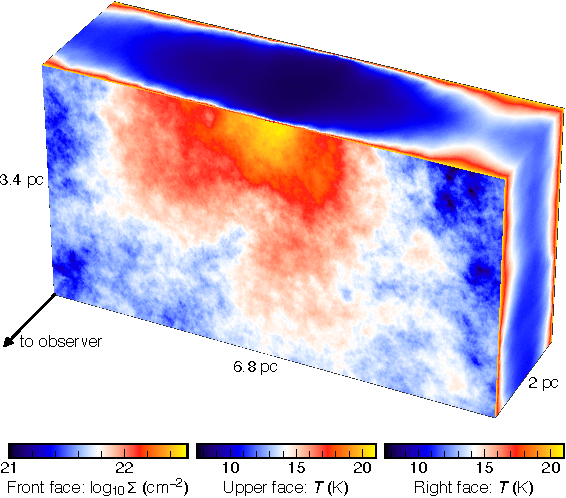
\includegraphics[width=0.98\columnwidth]{fig_cube3d.pdf}
\caption{A cut-away view of the radiative transfer model of the cloud, seen from the side of the observer. The front face is the
surface density map of the lower half of the imaged area, oriented as in Fig.~\ref{fig:simsky6}; the depth runs along the line of
sight. The upper face is a cut through the middle row of the map, and the right face a cut along its last column. Both show the
dust temperature in the plane of the cut.}
\label{fig:cube3d}
\end{figure}

\begin{figure*}[ht!]
\centering
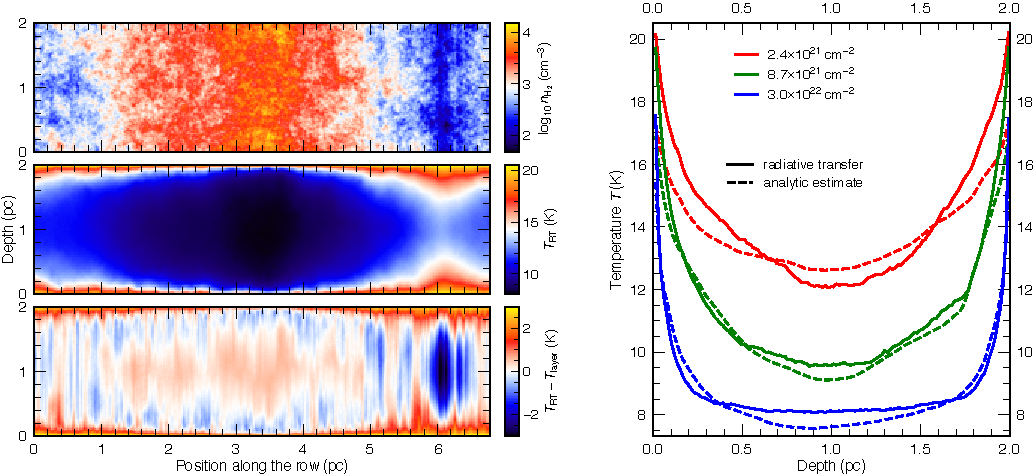
\includegraphics[width=0.98\textwidth]{fig_cube.pdf}
\caption{A slice through the radiative transfer model of the cloud, along the middle row of the map (horizontal axis) and the line
of sight (vertical axis). \emph{Left images}: The H$_2$ number density, the dust temperature, and the difference between the
dust temperature and that of the uniform layer with the same surface density in each column. \emph{Right panel}: The dust
temperature against the depth for three columns of different surface density, in the radiative transfer model (solid) and in the
analytic uniform layer (dashed).}
\label{fig:cube}
\end{figure*}

As a result, the emission of the model at $160${\um} is up to $1.5$ times that of the uniform layer with the same $\Sigma$. The
model has cells of $12{\arcsec}$, whereas the image of the simulated region has $3{\arcsec}$ pixels (Sect.~\ref{sec:modcloud}). The
emission in each pixel was therefore computed analytically for a uniform layer with its $\Sigma$ (Sect.~\ref{sec:factor}) and
multiplied in each band by the ratio of the emission of the model to that of the layer, interpolated from the cells to the pixels.

\section{Structure along lines of sight}
\label{app:arrange}

The fit of each pixel is biased by the whole distribution of dust temperatures along its line of sight. The correction method
(Sect.~\ref{sec:factor}) replaces this distribution by that of a single uniform body with the same $\Sigma$.

\subsection{Spheres and layers as extreme shapes}
\label{app:shape}

\begin{figure*}[ht!]
\centering
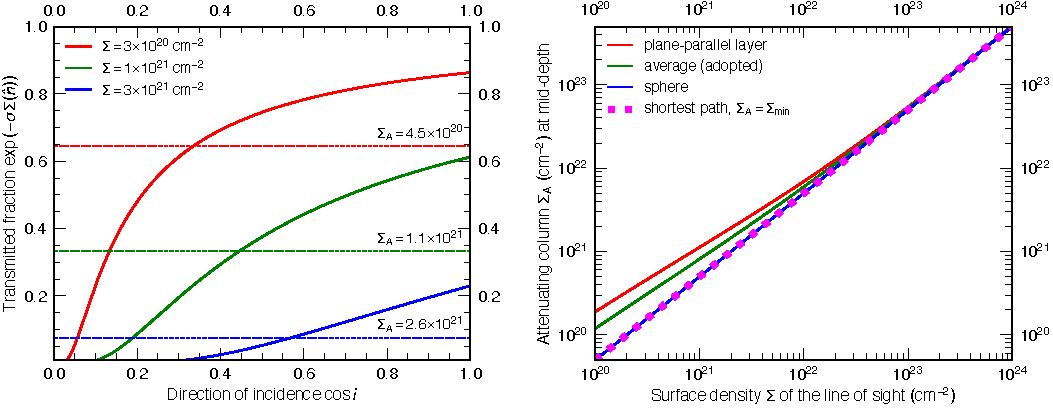
\includegraphics[width=0.95\textwidth]{fig_angular.pdf}
\caption{\emph{Left}: Transmitted fraction $\exp\left(-\sigma\Sigma(\hat n)\right)$ of the external radiation against the cosine of
the angle $i$ to the normal, for a dust grain at mid-depth of a plane-parallel layer of three total surface densities. The dashed
lines
mark the angular means of the curves and are labeled with the effective attenuating column $\Sigma_{\rm A}$ of Eq.~(\ref{eq:seff})
that gives the same mean intensity. \emph{Right}: Effective attenuating column $\Sigma_{\rm A}$ against the total
surface density $\Sigma$ of the line of sight, for the two extreme shapes and their adopted average, with the shortest-path column
$\Sigma_{\rm min}$ for comparison.}
\label{fig:angular}
\end{figure*}

The cylinder in Fig.~\ref{fig:relation} shows that the correction factors for the sphere and the layer are indeed the lower and
upper limits for other shapes. A cylinder is bounded across its axis, like a sphere, and unbounded along it, like a layer. Its
factor lies between them at every surface density, within $5$\% of the sphere and within $6$\% of the layer. The layer is an
extreme case because it is unbounded across the line of sight. A whole band of directions near the plane of the layer delivers no
radiation, however thin the layer is (Fig.~\ref{fig:angular}). In a bounded body, the path to the boundary is finite in every
direction, and every
direction delivers some radiation. The sphere is the opposite extreme: a compact body with a given central surface density blocks
less of the sky than any other body with that surface density. Uniform bodies of other shapes are bounded in some directions and
extended in others, and their correction factors lie between the
two limits. The method averages the attenuating columns of the two limiting shapes (Sect.~\ref{sec:factor}), so the error due to
the shape of a uniform body is at most ${\sim}5$\%. The surface layers of an extended cloud (Sect.~\ref{sec:diffuse}) and the
concentration of the material (Appendix~\ref{app:concentr}) can move the required factor outside these limits.

\subsection{Centrally concentrated structures}
\label{app:concentr}

In a layer, the density profile has no effect on $f$ (Sect.~\ref{sec:orient}). In a bounded body, slanted paths from a grain away
from the center cross the body along chords at
larger radii, so their columns depend on the density profile. Concentration of material can act only through these paths. The
effect was measured on a sphere with the density $\rho(r) \propto (1 + r^2/a^2)^{-1}$ out to its boundary. The sphere was
normalized so that the column through its center equaled the surface density $\Sigma$ of the uniform sphere it was compared with,
and $a$ was set by the central-to-edge density ratio. The positions along the central line of sight were weighted by the density
there, as in the emission. For each position, the column was integrated along the ray to the boundary in every direction of the
average.

\begin{table}[ht!]
%%%%% -----------------------------------------------------------------------------------------------------------------------------
%%%%% NUMBERS (2026-10-20): Table tab:concentr, and the numbers of Appendix B on two components,
%%%%% from python/paper_numbers/superposition_numbers.py, which uses superposition_test.py and hicorrect2.py.
%%%%% -----------------------------------------------------------------------------------------------------------------------------
\caption{Correction factor required by the central line of sight of a sphere of the given central surface density, for four
central-to-edge density ratios $\rho_{\rm C}/\rho_{\rm E}$.}
\label{tab:concentr}
\centering
\begin{tabular}{lcccc}
\hline\hline
\noalign{\smallskip}
$\Sigma$ (cm$^{-2}$) & \multicolumn{4}{c}{$\rho_{\rm C}/\rho_{\rm E}$} \\
\noalign{\smallskip}
\cline{2-5}
\noalign{\smallskip}
 & $1$ & $10$ & $10^2$ & $10^3$ \\
\hline
\noalign{\smallskip}
$5{\times}10^{21}$ & $1.093$ & $1.133$ & $1.169$ & $1.189$ \\
$1{\times}10^{22}$ & $1.276$ & $1.335$ & $1.409$ & $1.460$ \\
$3{\times}10^{22}$ & $1.699$ & $1.756$ & $1.892$ & $2.039$ \\
$1{\times}10^{23}$ & $1.835$ & $1.881$ & $1.981$ & $2.165$ \\
\noalign{\smallskip}
\hline
\end{tabular}
\end{table}

Table~\ref{tab:concentr} shows that the concentration always raises the required correction, because the mass of a concentrated
structure lies where the shielding is deepest. For a density ratio of $10$ the effect is $2$--$5$\% and for a ratio of $10^3$ it
is $9$--$20$\%. It is one-sided: on the central line of sight, a correction built on uniform structures under-corrects a
concentrated structure
and never over-corrects it.

\subsection{Two superposed components}
\label{app:twocomp}

This case of a denser structure at an unknown depth in a cloud was modeled as a
plane-parallel cloud of surface density $\Sigma_{\rm L}$ with an embedded uniform sphere of central surface density $\Sigma_{\rm
S}$. A direction is defined by its angle $\psi$ to the line of sight, measured from the direction toward the observer. The material
at the column depth $x$ in the cloud is shielded by the angular average of $x/|\cos\psi|$ toward the observer and of $(\Sigma_{\rm
L} - x)/|\cos\psi|$ away from the observer. A fraction $q$ of the cloud lies in front of every point of the sphere and the rest
behind it, so that the sphere lies between two layers of the cloud, in front of it for $q = 0$ and behind it for $q = 1$. A dust
grain at the position $z$ along the diameter of the sphere, from $-1$ to $1$ in units of its radius and positive toward the
observer, is shielded by the sphere over the path
\begin{equation}
   p(z,\psi) = -z\cos\psi + \left(1 - z^2\sin^2\psi\right)^{1/2},
\label{eq:lsphere}
\end{equation}
which contains the column $(\Sigma_{\rm S}/2)\,p(z,\psi)$. Beyond the sphere, the path also crosses the column $q\,\Sigma_{\rm
L}/|\cos\psi|$ of the cloud toward the observer or $(1-q)\,\Sigma_{\rm L}/|\cos\psi|$ away from the observer. The sum of the two
columns entered the angular average of Eq.~(\ref{eq:seff}), computed over $\psi$ with the weight $\sin\psi$, proportional to the
solid angle of the directions at that angle. The temperature of every grain along the line of sight was determined from
Eq.~(\ref{eq:law}). The emissions of the cloud and of the sphere, given by Eq.~(\ref{eq:emission}) with $\Sigma_{\rm L}$ and
$\Sigma_{\rm S}$ and the temperatures of their grains, were added, and one modified blackbody was fitted to the sum, exactly as for
the uniform bodies of Sect.~\ref{sec:factor}. This gave $\Sigma_{\rm F}$ of the composite line of sight, whose true value is
$\Sigma = \Sigma_{\rm L} + \Sigma_{\rm S}$, and the corrected value $f(\Sigma_{\rm F})\,\Sigma_{\rm F}$, with $f$ of
Eq.~(\ref{eq:factor}).

\begin{figure*}[ht!]
\centering
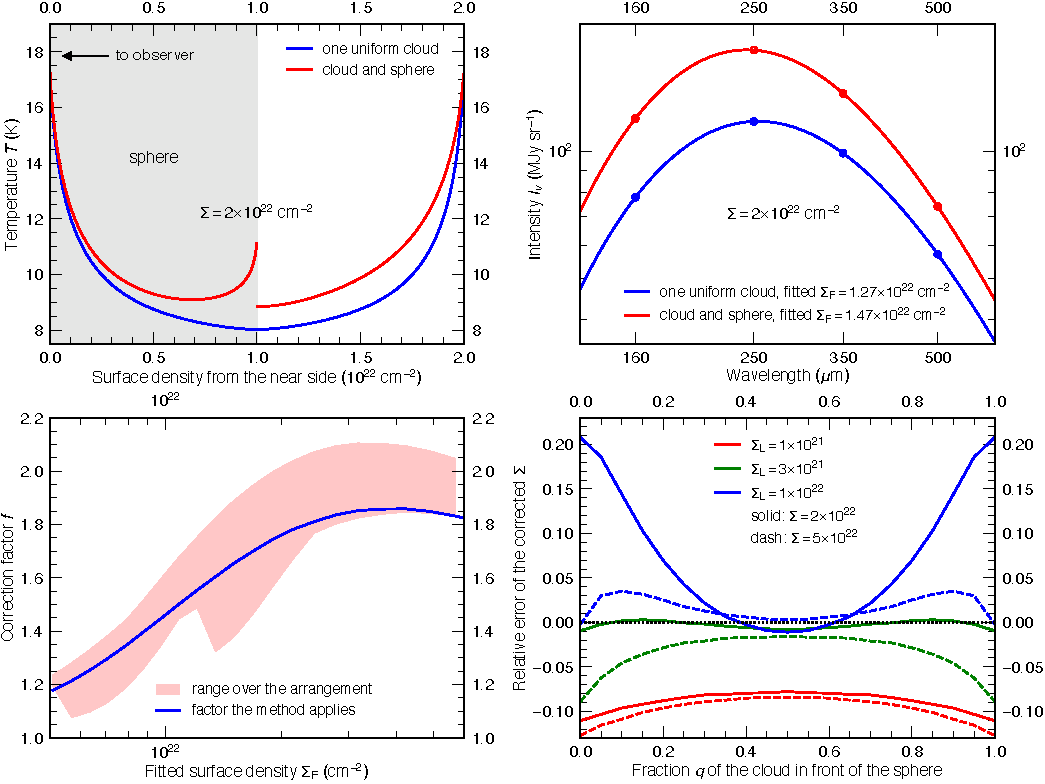
\includegraphics[width=0.95\textwidth]{fig_superposition.pdf}
\caption{Superposition of a cloud and a sphere (total $\Sigma = 2{\times}10^{22}$\,cm$^{-2}$). \emph{Upper left}: The dust
temperature along a line of sight through the uniform cloud that the method assumes (blue) and through the same surface density
divided equally between the cloud and a uniform sphere outside it, touching its near side (red, $q = 0$). \emph{Upper right}: The
intensities $I_{\lambda}$ of the two cases, with the surface densities $\Sigma_{\rm F}$ from a single modified blackbody fit.
\emph{Lower left}: The correction factor $f$ that the method applies and the range of factors that the composite lines of sight
require, against $\Sigma_{\rm F}$. The range covers cloud surface densities $\Sigma_{\rm L}$ of $10^{21}$, $3{\times}10^{21}$, and
$10^{22}$\,cm$^{-2}$ and all positions of the sphere. \emph{Lower right}: Relative errors of the corrected surface density against
the fraction $q$ of the cloud in front of the sphere, for three surface densities $\Sigma_{\rm L}$ of the cloud and total $\Sigma$
of $2{\times}10^{22}$ and $5{\times}10^{22}$\,cm$^{-2}$.}
\label{fig:superposition}
\end{figure*}

%%%%% -----------------------------------------------------------------------------------------------------------------------------
%%%%% NUMBERS (2026-10-20): from python/paper_numbers/superposition_numbers.py (range of the error over q; the worked example:
%%%%% q = 0, Sigma = 2e22, Sigma_cl = 1e22 cm^-2).
%%%%% -----------------------------------------------------------------------------------------------------------------------------
Figure~\ref{fig:superposition} shows the effect and its size. The example has a cloud and a sphere of equal surface densities,
$\Sigma_{\rm L} = \Sigma_{\rm S} = 10^{22}$\,cm$^{-2}$, totaling $\Sigma = 2{\times}10^{22}$\,cm$^{-2}$. The sphere lies outside
the cloud and touches its near side ($q = 0$). It is heated from the front and from the sides, where nothing blocks the incoming
radiation. Therefore, this line of sight is warmer and brighter than that through the uniform body with the same total $\Sigma$.
The fit returns $\Sigma_{\rm F} = 1.47{\times}10^{22}$\,cm$^{-2}$, against $1.27{\times}10^{22}$\,cm$^{-2}$ for the uniform body,
whose correction factor $1.57$ restores the true total $\Sigma$. To the composite line of sight, the method applies the factor of a
uniform body with $\Sigma_{\rm F} = 1.47{\times}10^{22}$\,cm$^{-2}$, $1.64$ instead of the required $1.36$, and obtains
$2.4{\times}10^{22}$\,cm$^{-2}$, overestimated by $21$\%.

Figure~\ref{fig:superposition} also gives the general picture. The factors that the composite lines of sight require
form a band around the factor that the method applies, and the error of the corrected surface density ranges from $-13$ to $+21$\%.
Its sign depends on the cloud. A tenuous cloud ($\Sigma_{\rm L} = 10^{21}$\,cm$^{-2}$) holds only $5$\% of the total $\Sigma =
2{\times}10^{22}$\,cm$^{-2}$, but
its dust is warm. Its emission raises the fitted temperature of the line of sight, from $11.4$\,K for an isolated sphere to
$11.7$--$12.0$\,K, which lowers $\Sigma_{\rm F}$. The correction is then too small by $8$--$13$\%, at any depth, although an
isolated sphere would be corrected $2$\% too much. A dense cloud ($\Sigma_{\rm L} = 10^{22}$\,cm$^{-2}$) with the sphere at one of
its sides makes the line of sight warmer
than a single body, and the correction is then too large, by up to $21$\%. When the sphere lies near the middle of a dense cloud,
the error is only a few percent. The simulated star-forming region of Sect.~\ref{sec:sim}, built entirely from radiative transfer
models, shows both regimes: the wings of filaments in its tenuous outer areas are corrected too little, and the flanks of filaments
in its dense central areas too much.

\section{Calibration for different radiation fields}
\label{app:field}

The correction was tested on the grid of models in nine radiation fields (Appendix~\ref{sec:grid}), comparing for every pixel the
factor that the correction applies with the factor that restores its true surface density. Without the field factor, the errors
range from $-23$ to $+26$\% (Fig.~\ref{fig:fielderr}). They change sign twice: the correction is too large in the weakest fields,
too small for $G_0 \approx 20$--$100$, and again too large at the highest surface densities in the strongest fields.

\begin{figure*}[ht!]
%%%%% -----------------------------------------------------------------------------------------------------------------------------
%%%%% NUMBERS (2026-11-05): Figure fig:fielderr, upper: Eq. (5) with the constants of python/paper_numbers/laws_refit.txt (refit.py
%%%%% on hires/attenuation_law_G0=*.txt, the tables of fit_attenuation_law.py, refitted with wide limits; table3.dat at the CDS).
%%%%% Lower: python/paper_numbers/field_factor_errors.py on the histograms harvest_calib3_G0=*.txt.hist.npz written by
%%%%% harvest_calib3.py (binned, so accurate to about 1 percent); the unrounded values are in field_factor_errors.txt. Both panels
%%%%% are plotted by fig_field_errors in make_hires2_figures12.py. The errors for a local field that differs by a factor of 2.2 or
%%%%% 4.7 (Sect. 7) are the differences of the 'without g' values of the fields one or two steps from G_0 = 10 from those at
%%%%% G_0 = 10. The decomposition of g is from analytic_g.py and scale_test.py with hicorrect2.py.
%%%%% -----------------------------------------------------------------------------------------------------------------------------
\centering
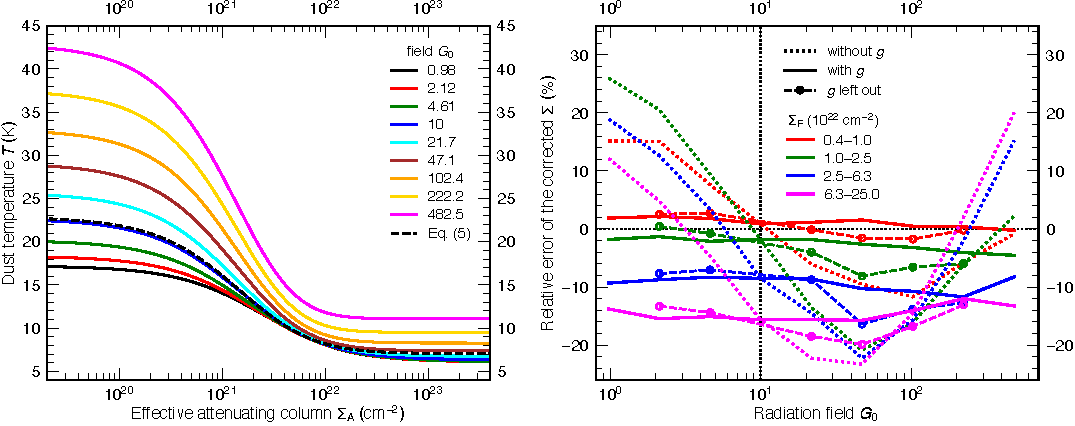
\includegraphics[width=0.96\textwidth]{fig_field_errors.pdf}
\caption{Temperature relations and errors of the correction for the grid of radiation fields. \emph{Left}: The relation
$T(\Sigma_{\rm A})$ of Eq.~(\ref{eq:law}) refitted on the models of each field strength $G_0$ is compared with the adopted relation
for $G_0 = 10$ (dashed line). \emph{Right}: Relative errors of the corrected surface density are plotted against $G_0$, in four
ranges of the fitted surface density $\Sigma_{\rm F}$. Each point is the median over the pixels in its range. The correction
without the field factor $g$ (dotted lines) is compared with that with $g$ of all nine fields (Sect.~\ref{sec:g0corr}, solid
lines). Each circle on the dashed lines is a separate test of a field $G_0$ with $g$ interpolated in $\log G_0$ between its two
neighboring values, the field itself being left out. Such a test is not possible for the weakest and strongest fields and for the
field $G_0 = 10$ of the calibration (vertical dotted line). In all cases, the correction factor $f_{G_0}$ is that of
Eq.~(\ref{eq:factorg0}), with $g = 1$ for the dotted lines.}
\label{fig:fielderr}
\end{figure*}

\subsection{Deriving the field factor $g$}
\label{app:fieldR}

Each field shifts the plateaus of the envelopes to a different $\Sigma_{\rm F}$, so bins of $\Sigma_{\rm F}$ would compare
unrelated pixels in different fields. The pixels were therefore binned in their true $\Sigma$, in bins of $0.05$\,dex. Each bin gave
the
mean $\log\Sigma_{\rm F}$ and the mean logarithm of the required factor $\Sigma/\Sigma_{\rm F}$, which was smoothed against
$\log\Sigma_{\rm F}$ and divided by the same at $G_0 = 10$.

With the field factor $g$, the errors are within $4$\% of those at $G_0 = 10$ (the errors of the calibration itself) in every field
and range of $\Sigma_{\rm F}$ (Fig.~\ref{fig:fielderr}). This agreement is not an independent test, because $g$ was derived from
the same models. When a field is left out of the calculation of $g$, its errors change by
up to $6$\% from those with $g$ and by up to $8$\% from those at $G_0 = 10$, which measures the error of interpolating between the
fields of the model grid.

The shape of $g(\Sigma_{\rm F}, G_0)$ follows from the changes of the relation of Eq.~(\ref{eq:law}) with the field, refitted on
the models of each field (Fig.~\ref{fig:fielderr}), whose constants are available at the CDS. For $G_0 = 10$, they differ from
those of Eq.~(\ref{eq:law}), which was fitted to the main grid and the filaments, so only their trends with the field are discussed
here. $T_{\rm max}$ rises steadily with increasing $G_0$, whereas $T_{\rm min}$ stays near $6$--$7$\,K up to $G_0 \approx 20$ and
then rises, while the shielded dust is heated by the infrared emission of the warmer dust around it. The contrast $T_{\rm
max}/T_{\rm min}$ therefore increases from $2.8$ to about $4$ near $G_0 \approx 50$--$100$ and then decreases slightly. The higher
$T_{\rm max}$ and the steeper decline of $T(\Sigma_{\rm A})$ increase the bias and dominate up to $G_0 \approx 50$. The higher
$T_{\rm min}$ and the overall warming reduce the underestimation of $\Sigma$ in the strongest fields. The analytic calculation of
Sect.~\ref{sec:factor} with the refitted relations reproduces these features only qualitatively, within $25$\%, because the density
in the bodies of the calculation is uniform, whereas the models are centrally concentrated. The derived $g$, which describes only
the change with the field and leaves the calibration at $G_0 = 10$ unchanged, was therefore adopted.

\subsection{Estimating the radiation fields of clouds}
\label{app:fieldest}

The field strength of a cloud is estimated by comparing its fitted temperatures with those of the models at the same surface
density. Both come from the images $\Dim_{13.5}$ and $\mathcal{T}_{13.5}$ that \emph{hires} derived from the \emph{Herschel} images
of the cloud and from the simulated images of the models in the grid of radiation fields (Appendix~\ref{sec:grid}). For each field
$G_0$ of the grid, the median temperature of the model pixels was tabulated in bins of $0.2$\,dex of the fitted surface density. At
a fixed surface density, this temperature rises monotonically with $G_0$. The temperature in each pixel of the image
$\mathcal{T}_{13.5}$ of a cloud is therefore converted into a field strength, by interpolating $\log G_0$ against the median
temperature of the models in the same bin of surface density. The procedure is built into \emph{hicorrect}, which applies it
whenever the temperature image is given and the field strength is not specified.

The scaling relation $T \propto G_0^{1/6}$ \citep{IvezicElitzur1997, Tielens2005} holds only for dust that is optically thin to the
heating radiation. At a fixed $\Sigma_{\rm F}$, the models give $T_{\rm F} \propto G_0^{\,0.09\text{--}0.13}$, so the scaling
relation would place a cloud at a field several times too weak.

The parameter $G_0$ is estimated from the diffuse material only, between $10^{21}$ and $6.31{\times}10^{21}$\,cm$^{-2}$. In denser
bins, the $G_0$ values that the procedure gives rise steadily with the surface density in every observed cloud. In Aquila, for
example, the median $G_0$ rises from about $20$--$40$ in the diffuse bins to more than $100$ in the densest ones. The rise of $G_0$
is found even in Scorpius, which contains no strong heating source. It is therefore not a real increase of the field strength but a
bias. Indeed, a dense structure seen through warm diffuse material has a higher fitted temperature than an isolated core of the
same surface density, and the procedure attributes the extra warmth to the field. Pixels warmer than the models in the strongest
field of the grid are counted separately. They are heated either internally by protostars or externally by nearby massive stars,
beyond the range of the grid.

The resulting field strength $G_0$ of a cloud is defined as the median of the $G_0$ values of its diffuse bins, weighted by the
number of pixels. The fields at the 16th and 84th percentiles of the temperature give its spread. Table~\ref{tab:g0regions} lists
the results for nine observed regions. Only Scorpius and Orion~A are close to the value $G_0 = 10$ of the calibration. In Taurus,
the diffuse dust ($13.6$--$14.4$\,K between $10^{21}$ and $2.5{\times}10^{21}$\,cm$^{-2}$) is colder than the models in the
weakest field of the grid ($14.9$\,K), and the procedure gives only an upper limit. The correction then uses $G_0 = 0.98$, which
changes the corrected $\Sigma$ by a few percent at most (Fig.~\ref{fig:fielderr}).

\begin{table}[ht!]
\caption{Estimates of $G_0$ for nine regions observed with \emph{Herschel}.}
\label{tab:g0regions}
\centering
\begin{tabular}{lcccc}
\hline\hline
\noalign{\smallskip}
Cloud & $G_{0,16}$\tablefootmark{a} & $G_{0,50}$\tablefootmark{a} & $G_{0,84}$\tablefootmark{a} & Too warm\tablefootmark{b} \\
\noalign{\smallskip}
\hline
\noalign{\smallskip}
Taurus      &\phantom{0}$^<$0.98             &\phantom{0} $^<$0.98 &\phantom{0} $^<$0.98 & \phantom{0}0.0 \\
California  &\phantom{0} 3.6                &\phantom{0} 5.4     &\phantom{0} 6.9     & \phantom{0}0.1 \\
Perseus     &\phantom{0} 3.2                &\phantom{0} 4.7     &\phantom{0} 6.1     & \phantom{0}0.1 \\
Scorpius    &\phantom{0} 6.2                &\phantom{0} 7.9     & 10\phantom{0}      & \phantom{0}0.0 \\
Orion~A     &\phantom{0} 5.9                &\phantom{0} 8.9     & 28\phantom{0}      & \phantom{0}2.0 \\
Ophiuchus   & 14\phantom{0}                 & 31\phantom{0}      & 55\phantom{0}      & \phantom{0}0.7 \\
Aquila      & 25\phantom{0}                 & 33\phantom{0}      & 41\phantom{0}      & \phantom{0}0.4 \\
W3 W4 W5    & 54\phantom{0}                 & 62\phantom{0}      & 73\phantom{0}      & \phantom{0}1.3 \\
Cygnus~X    & 200\phantom{0}\phantom{0}     & 250\phantom{0}\phantom{0}     & 320\phantom{0}\phantom{0}     & 21.8           \\
\noalign{\smallskip}
\hline
\end{tabular}
\tablefoot{
\tablefoottext{a}{Fields that reproduce the 16th, 50th, and 84th percentiles of the fitted temperature, as medians over the diffuse
bins between $10^{21}$ and $6.31{\times}10^{21}$\,cm$^{-2}$ weighted by their pixels (Appendix~\ref{app:fieldest}); $G_{0,50}$ is
taken as the field of the region. The values preceded by "$^<$" are upper limits, below the weakest field of the grid.}
\tablefoottext{b}{Percentage of all pixels of the map warmer than the models in the strongest field of the grid.}
}
\end{table}

%%%%% NUMBERS (2026-11-09): estimate_field of hicorrect2.py on hi.surface.density.r13p5.fits and hi.temperature.r13p5.fits of
%%%%% hires/simsky6_RT_enh_cirronly (8.82; 7.29 and 10.88) and hires/simsky6_RT_enh_cirrdepth=2_nocrater (4.33; 2.75 and 6.08).
The procedure was tested on the simulated star-forming region (Sect.~\ref{sec:modcloud}), computed for $G_0 = 10$. The image of
the cloud alone gives $G_0 = 8.8$, with $7.3$ and $10.9$ at the 16th and 84th percentiles of the temperature. The image of the
whole region, with its filaments and cores, gives $G_0 = 4.3$, with $2.7$ and $6.1$. The estimate is lower probably because the
diffuse bins contain the outer parts of filaments, which are colder than cloud material of the same surface density. The field
of a cloud rich in filaments may therefore be underestimated by a factor of about $2$, which is included in the uncertainties of
Appendix~\ref{sec:field}.

A single $G_0$ value per cloud is an approximation. In Orion~A and Ophiuchus, the fields at the 16th and 84th percentiles differ by
a factor of $4$--$5$, because parts of these regions are exposed to radiation from nearby OB stars. For such clouds, the map can be
divided into regions with their own $G_0$ values. In Cygnus~X, a fifth of the pixels are warmer than the models in the strongest
field, and the correction factor $f_{G_0}$ is not calibrated for them.

\section{Inadequacy of the observed colors and temperatures}
\label{app:onlysigma}

\subsection{Insufficient accuracy of the observed colors}
\label{app:colors}
\label{sec:amplification}

The temperature structure along a line of sight could, in principle, be measured by fitting more than one component to the observed
spectrum. Without noise, a free two-temperature fit $160$--$500${\um} recovers $0.96$--$1.00$ of the true surface density
$\Sigma$ at the centers of four models of cores, against $0.62$--$0.91$ for the single-temperature fit. The residuals of the
single-temperature fit, however, are only $1.0$--$5.8$\% (root-mean-square), positive at $160$ and $500${\um} and negative at
$250$ and $350${\um} (Fig.~\ref{fig:mixing}). The underestimation of $\Sigma$ is $6.6$--$8.9$ times larger, so any method that
infers it from the colors amplifies the photometric errors by that factor. With calibration uncertainties of $20$\% at $160${\um}
and $10$\% at $250$--$500${\um} \citep{Konyves+2015}, the residual pattern is below the photometric accuracy. The correction must
therefore be calibrated on models in which the answer is known.

\begin{figure*}[ht!]
\centering
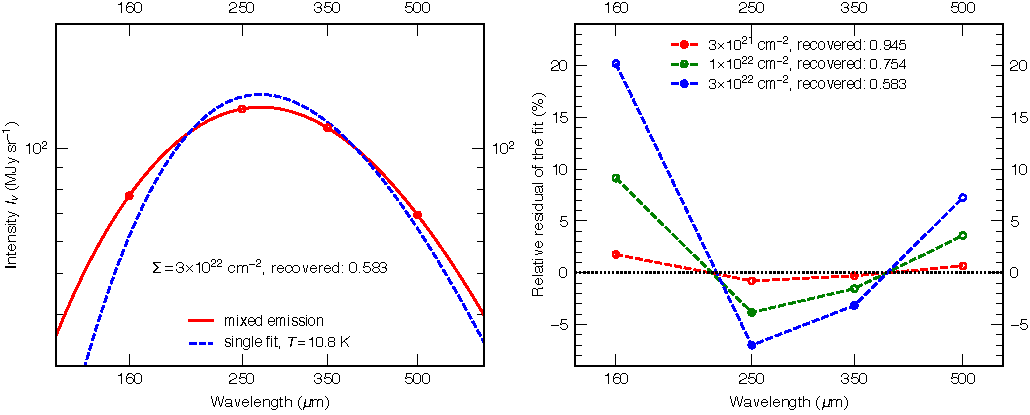
\includegraphics[width=0.95\textwidth]{fig_mixing.pdf}
\caption{Single-temperature fits to lines of sight through a mixture of temperatures. \emph{Left}: The emission of a line of
sight of $3{\times}10^{22}$\,cm$^{-2}$, summed over depth, with the single modified blackbody fitted to it in the four wavebands.
\emph{Right}: Relative residuals of the fit in each waveband for three surface densities, with the fraction of the true $\Sigma$
recovered. The residuals grow with the surface density but remain below the calibration uncertainties of $20${\%} at $160${\um} and
$10${\%} at the longer wavebands.}
\label{fig:mixing}
\end{figure*}

\subsection{Ambiguity of the fitted temperatures}
\label{app:tcorr}

A fitted temperature that differs from the one that the relation predicts at the same surface density might improve the correction.
Four corrections that use it were tested, as tables or functions of the surface density and the temperature, calibrated on the
radiative transfer models or on analytic lines of sight. They changed the median core mass by only $2$--$9$\%, less than the mass
errors caused by uncertain footprints and backgrounds (Appendix~\ref{app:footprint}). Each correction failed in some cases,
under-correcting dense material in stronger fields, over-correcting the flanks of filaments, or copying the noise of the finest
image into the factor.

The reason is that a warm pixel is ambiguous. A stronger radiation field makes it warmer and requires more correction, whereas a
pixel near the surface of a structure, or one whose line of sight crosses a warm cloud, is warmer but requires less. The models of
the calibration contain only the first case, the simulated star-forming region mostly the second, and the temperature of a single
pixel cannot distinguish them. Because the field varies over parsecs, much more slowly than the temperature across a filament,
$G_0$ is estimated as one number for a cloud from the diffuse material of the whole map (Appendix~\ref{app:fieldest}).

\section{Uncertainties and limitations}
\label{sec:limits}

\begin{table*}[ht!]
%%%%% -----------------------------------------------------------------------------------------------------------------------------
%%%%% NUMBERS (2026-10-20): the values of this table are copied from Sects. 5, 6 and 7 and Appendices B and D; see comments there.
%%%%% -----------------------------------------------------------------------------------------------------------------------------
\caption{Accuracy of surface densities and masses derived from \emph{Herschel} images at $160$--$500${\um}.}
\label{tab:accuracy}
\centering
\setlength{\tabcolsep}{4pt}
\begin{tabular}{llll}
\hline\hline
\noalign{\smallskip}
Quantity\tablefootmark{a} & Uncorrected\tablefootmark{b} & Corrected\tablefootmark{c} & Models (Section)\tablefootmark{d} \\
\noalign{\smallskip}
\hline
\noalign{\smallskip}
\multicolumn{4}{l}{\emph{Errors of the method}} \\
total $\Sigma$ within core footprints, accuracy ratio      & 0.78 (0.56--0.93) & 0.99 (0.92--1.03) & 1815 cores (\ref{sec:valgrid}) \\
core mass $M$ from the image, accuracy ratio               & 0.63 (0.46--0.86) & 0.98 (0.75--1.11) & 1750 cores (\ref{sec:valgrid}) \\
core center $\Sigma$ (within $3{\arcsec}$), relative error & $-0.44$          & $-0.13$           & 1815 cores (\ref{sec:valgrid}) \\
filament crest $\Sigma$, accuracy ratio                    & 0.42--0.86        & 0.78--0.94        & 7 filaments (\ref{sec:cyl}) \\
filament linear density $\Lambda$, accuracy ratio          & 0.60--0.96        & 0.93--1.01        & 7 filaments (\ref{sec:cyl}) \\
filament width $H_{13.5}$ (true $48{\arcsec}$), accuracy ratio & 1.21--1.65   & 1.15--1.31        & 6 filaments (\ref{sec:cyl}) \\
filament slope $\alpha_{13.5}$, error                      & up to $-0.22$     & within $\pm 0.05$ & 7 filaments (\ref{sec:cyl}) \\
diffuse cloud, accuracy ratio of $\Sigma$                  & 0.76              & 0.89 (0.86--0.94) & cloud model (\ref{sec:sim}) \\
filament flanks in a dense cloud, relative error           & --                & $0.10$--$0.16$    & simulated region (\ref{sec:sim}) \\
superposed structures, relative error of $\Sigma$          & --                & $-0.13$ to $0.21$ & analytic (\ref{app:twocomp}) \\
field $G_0 = 1$ to 483 with $g$, relative error            & --                & $-0.16$ to $0.02$ & 9 radiation fields (\ref{sec:field}) \\
inclined layers, random, mean relative error               & --                & $0$--$0.23$     & analytic (\ref{sec:incl}) \\
inclined filaments, random, mean relative error            & --                & $0$--$0.08$     & analytic (\ref{sec:incl}) \\
\noalign{\smallskip}
\multicolumn{4}{l}{\emph{Additional errors from uncertain parameters and data}} \\
local field wrong by a factor of 2.2, relative error       & --                & $-0.12$ to $0.12$ & 9 radiation fields (\ref{sec:field}) \\
floor $T_{\rm min}$ wrong by $\pm 1$\,K, relative error    & --                & $-0.22$ to $0.51$ & relation (\ref{sec:floor}) \\
calibration error of 10\% at 500{\um}, $\Sigma$            & 0.16--0.18        & 0.16--0.23        & uniform bodies (\ref{sec:calerr}) \\
\noalign{\smallskip}
\hline
\end{tabular}
\tablefoot{
\tablefoottext{a}{Accuracy ratios are measured over true values. Values are medians over the models, with the 16th and 84th
percentiles in parentheses where available; ranges span the models listed. For the diffuse cloud, the range is that between
$10^{21}$ and $10^{22}$\,cm$^{-2}$.}
\tablefoottext{b}{The derived $\Dim_{13.5}$ from \emph{hires}, or a single modified blackbody fit.}
\tablefoottext{c}{The same after the correction of Eq.~(\ref{eq:correction}).}
\tablefoottext{d}{The radiative transfer or analytic models on which the quantity was measured, with the section that describes the
test.}
}
\end{table*}

\subsection{Summary of the accuracy}
\label{sec:accuracy}

Table~\ref{tab:accuracy} collects the accuracies measured on noiseless models with simple backgrounds, before and after the
correction.
%%%%% NUMBERS (2026-11-10): quadrature sums of the rows of Table tab:accuracy. Method alone: diffuse sqrt(0.11^2+0.17^2) = 0.20,
%%%%% dense sqrt(0.13^2+0.21^2) = 0.25 (cloud 0.89, core center -0.13, superposition -0.13 to 0.21). Total adds G0 (0.12),
%%%%% calibration (0.17, 0.23), and T_min (small below 1e22, up to 0.51 above): ~0.30 and ~0.5.
The errors of the method itself, obtained with the true dust properties and radiation fields, combine in quadrature the
underestimation that the correction leaves and the superposition of structures. They are ${\sim}20$\% in diffuse material and
${\sim}25$\% in dense structures. A realistic total adds a local $G_0$ that differs from that of the cloud by a factor of ${\sim}2$,
the calibration uncertainty of \emph{Herschel}, and an error of $1$\,K in the floor temperature $T_{\rm min}$. The total is
${\sim}30$\% in diffuse material and ${\sim}50$\% in dense structures, where the floor is the largest term. Uncorrected images
systematically underestimate $\Sigma$ by $10$--$25$\% in diffuse material and by factors of $1.3$--$2.4$ in dense structures, and
they also have the calibration uncertainty. The total error of $30$--$50$\% in the corrected $\Sigma$ corresponds to ${\sim}2$\,K
in the corrected temperature (Eq.~(\ref{eq:sensitivity})), whereas the fitted temperatures are overestimated by $1$--$4$\,K in dense
structures. These estimates hold for fields within the grid of models and for lines of sight without internal heating. In addition,
the absolute dust opacity is uncertain by a factor of $1.5$--$2$ \citep{Roy+2014} and may increase in dense cores
\citep{Ossenkopf+Henning1994, Juvela+2015}.

\subsection{Errors of core footprints}
\label{app:footprint}

In observed images, the footprints of cores, estimated by source extraction, can be inaccurate. A footprint radius $R$ too small by
$\Delta R/R = 0.25$ or $0.5$ lowers the median corrected mass from $0.98$ to $0.83$ or $0.52$, because part of the core is counted
as background (Fig.~\ref{fig:footprint}). A footprint too large by $0.25$ or $0.5$ raises it to $1.06$ or $1.11$, and much more for
cores of low contrast, whose mass is small compared with the background within the footprint. For contrasts below $1.5$, a
footprint twice too large triples the median mass. These errors are lower limits, because real cores overlap with other structures,
and because the true masses of the tests were measured with the same background just outside the footprint. An embedded core has a
crater-like background, because the lines of sight through the core cross less of the
surrounding cloud than those next to it, and a background taken just outside the core is overestimated. This underestimates the
masses
of resolved cores by factors of up to $1.4$--$1.8$ in filaments \citep{Menshchikov2016}.

\begin{figure}
\centering
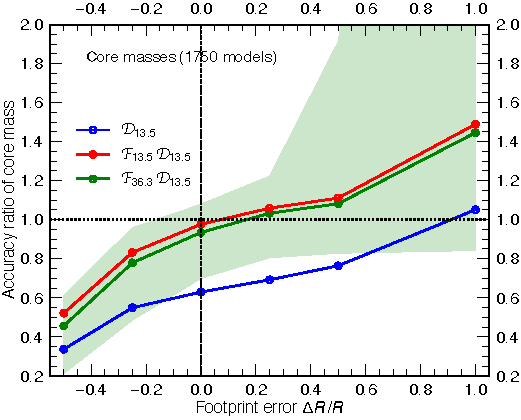
\includegraphics[width=0.95\columnwidth]{fig_footprint.pdf}
\caption{The accuracy ratio of the core mass for the $1750$ models of the subdivision grid in which it can be measured, when the
estimated radius $R$ of the core, and hence of its footprint, is too small ($\Delta R < 0$) or too large ($\Delta R > 0$). The
background is always taken in a ring just outside the footprint used. The lines are medians over the models, and the band marks
the 16th to 84th percentiles for $\mathcal{F}_{36.3\,}\mathcal{D}_{13.5}$.}
\label{fig:footprint}
\end{figure}

\subsection{Uncertainty of the radiation field}
\label{sec:field}

%%%%% -----------------------------------------------------------------------------------------------------------------------------
%%%%% NUMBERS (2026-11-05): from Figure fig:fielderr (see the comment there).
%%%%% -----------------------------------------------------------------------------------------------------------------------------
With the field factor $g$, the errors of the surface density correction in the nine radiation fields of the grid are within $4$\%
of those at $G_0 = 10$ (Appendix~\ref{app:field}). In Aquila, the field factor varies by only $\pm 3$\% between the values of $G_0$
at the 16th and 84th percentiles of the temperature of the diffuse material (Appendix~\ref{app:fieldest}). A local $G_0$ that
differs from that of the cloud by a factor of $2.2$ or $4.7$ changes the corrected $\Sigma$ by $-12$ to $12$\% or $-19$ to $22$\%,
respectively (Fig.~\ref{fig:fielderr}).
%%%%% These are the differences between the dotted lines at G0 = 4.61 and 21.7, or 2.12 and 47.1, and those at G0 = 10. The estimate of $G_0$ for a structured cloud can be underestimated by the first of these factors
(Appendix~\ref{app:fieldest}).

\subsection{Inclined layers and filaments}
\label{sec:incl}

%%%%% -----------------------------------------------------------------------------------------------------------------------------
%%%%% NUMBERS (2026-10-20): from python/paper_numbers/inclination_errors.py (the adopted factor of hicorrect2.py, G_0 = 10).
%%%%% -----------------------------------------------------------------------------------------------------------------------------
The factor was computed for lines of sight normal to a plane-parallel layer or perpendicular to the axis of a cylindrical filament.
Seen at an angle $i$ from that direction, a layer or a filament has the same temperature profile along the line of sight, but both
$\Sigma$ and $\Sigma_{\rm F}$ are larger by the factor $(\cos i)^{-1}$. The correction factor that it requires does not change,
whereas the correction applies the factor of a denser structure. The corrected $\Sigma$ is then overestimated by up to $27$\% at $i
= 70\degr$. For isotropic orientations,
the inclinations of layers and filaments are uniformly distributed in $\cos i$ and $\sin i$, respectively. Averaged over these
distributions, the error is up to $23$\%
for layers and up to $8$\% for filaments. Both maxima lie between $3.2{\times}10^{21}$ and $10^{22}$\,cm$^{-2}$, where the factor
rises most steeply (Fig.~\ref{fig:relation}). For real clouds, which are rarely extended thin layers, the error is probably smaller.

\subsection{Floor temperature of shielded dust}
\label{sec:floor}

The factor is very sensitive to the temperature $T_{\rm min} = 7.0$\,K that dust approaches when it is completely shielded
(Eq.~(\ref{eq:law})). Lowering $T_{\rm min}$ by $1$\,K raises the factor by $30$\% at $10^{22}$\,cm$^{-2}$ and by $51$\% at
$3{\times}10^{22}$\,cm$^{-2}$, and raising it by $1$\,K lowers the factor by $13$ and $22$\%. The fit to $2086$ spheres and seven
cylinders constrains $T_{\rm min}$ well (Fig.~\ref{fig:shielding}), and other radiative transfer models of prestellar cores give
similar central temperatures of $7$--$8$\,K in the local radiation field \citep{Evans+2001, Zucconi+2001}.
The error of $1$\,K adopted in Appendix~\ref{sec:accuracy} is comparable to the differences among these models and to the
changes of $T_{\rm min}$ with the field (Appendix~\ref{app:fieldR}).

\subsection{Noise and calibration errors}
\label{sec:calerr}

The correction is insensitive to noise, because it evaluates a smooth function of an image and fits nothing: realistic Gaussian
noise changed the total corrected surface density by less than $0.5$\%. A calibration error affects
$\Sigma_{\rm F}$, and the corrected $\Sigma$ follows. An error of $10$\% at $500${\um}, the reference waveband, changes the
uncorrected $\Sigma$ by $16$--$18$\% and the corrected one by $16$--$23$\%. The correction enlarges the error by up to $1.4$ times
only where $f$ rises steeply, between
$10^{22}$ and $3{\times}10^{22}$\,cm$^{-2}$.

\subsection{Internally heated sources}
\label{sec:notdo}

A line of sight through a protostar contains an internal source and has a reversed temperature gradient, so the accuracy of the
correction there is unknown. Every pixel was nevertheless corrected, because the correction would otherwise depend on a source
extraction. The masses of protostellar cores
measured in corrected images should therefore be used with caution.

\end{document}
